\documentclass{article}

\usepackage[labelformat=empty]{caption}
\usepackage[most]{tcolorbox}
\usepackage{capt-of}
\usepackage{changepage, amsmath, amssymb, pgfplots, tikz}
\usepackage{colortbl}
\usepackage{darkmode}
\usepackage{fullpage}
\usepackage{graphicx}
\usepackage{pst-eucl}
\usepackage{tabularx}
\usepackage{tikz-3dplot}
\usepackage{tkz-euclide}
\usepackage{ulem}

%  === Enable dark mode ===
%  Comment the line below to switch to light mode.
%  Note that some figures will keep a dark background, I might (!) fix this issue later.
\enabledarkmode

%  === Define custom color ===
\definecolor{myamber}{HTML}{ffc107}
\definecolor{myblue}{HTML}{2196f3}
\definecolor{mybluegray}{HTML}{607d8b}
\definecolor{mybrown}{HTML}{795548}
\definecolor{mycyan}{HTML}{00bcd4}
\definecolor{mydeeporange}{HTML}{ff5722}
\definecolor{mydeeppurple}{HTML}{673ab7}
\definecolor{mygray}{HTML}{9e9e9e}
\definecolor{mygreen}{HTML}{4caf50}
\definecolor{myindigo}{HTML}{3f51b5}
\definecolor{mylightblue}{HTML}{03a9f4}
\definecolor{mylightgreen}{HTML}{8bc34a}
\definecolor{mylime}{HTML}{cddc39}
\definecolor{myorange}{HTML}{ff9800}
\definecolor{mypink}{HTML}{e81e63}
\definecolor{mypurple}{HTML}{9c27b0}
\definecolor{myred}{HTML}{f44336}
\definecolor{myteal}{HTML}{009688}
\definecolor{myyellow}{HTML}{ffeb3b}
\definecolor{p1}{HTML}{caf0f8}
\definecolor{p2}{HTML}{ade8f4}
\definecolor{p3}{HTML}{90e0ef}
\definecolor{p4}{HTML}{48cae4}
\definecolor{p5}{HTML}{00b4d8}
\definecolor{p6}{HTML}{0096c7}
\definecolor{p7}{HTML}{0077b6}
\definecolor{p8}{HTML}{023e8a}
\definecolor{p9}{HTML}{03045e}
\definecolor{pag}{HTML}{293133}

% === Disable identation ===
\setlength{\parindent}{0pt}

%  === Plot settings ===
\pgfplotsset{compat=1.16}
\usetikzlibrary{3d,backgrounds,intersections}
\usetikzlibrary{arrows.meta}
\usetikzlibrary{arrows.meta}
\usetikzlibrary{calc,arrows.meta}
\usetikzlibrary{calc,patterns,angles,quotes}
\tikzset{
    conditional line/.style 2 args={
            /utils/exec={\pgfmathsetmacro{\xcoordA}{#1}},
            /utils/exec={\pgfmathsetmacro{\xcoordB}{#2}},
            insert path={
                    \ifdim\xcoordA pt>\xcoordB pt
                        (\xcoordA,0) -- (\xcoordB,0)
                    \fi
                },
        },
}

\psset{PointName=none,PointSymbol=none}

\usepgfplotslibrary{groupplots}
\usepgfplotslibrary{groupplots}

%  === Fix broken canvas is xy plane at z option ===
%  for more information, see: https://tex.stackexchange.com/a/48776/121799
\makeatletter
\tikzoption{canvas is xy plane at z}[]{% 
    \def\tikz@plane@origin{\pgfpointxyz{0}{0}{#1}}% 
    \def\tikz@plane@x{\pgfpointxyz{1}{0}{#1}}% 
    \def\tikz@plane@y{\pgfpointxyz{0}{1}{#1}}% 
    \tikz@canvas@is@plane}
\makeatother


\begin{document}

\textbf{Human Frequency Range} - Humans can only hear a set range of frequencies of sound. In addition, we have a set range of frequencies that we are more sensitive to.

\vspace{-10pt}
\begin{center}
	Audible Range: 20 Hz - 20 000 Hz \qquad Sensitive Range: 2000 Hz - 5000 Hz
\end{center}

\vspace{\baselineskip}

\textbf{Standing Waves} - When a wave is propagated in an environment where it can be reflected back to itself, it will have certain resonant frequencies where it takes on the appearance of a standing wave. A standing wave appears as though it is not moving in one direction, but rather oscillating back and forth.
\begin{center}
	\hspace*{-8pt}
	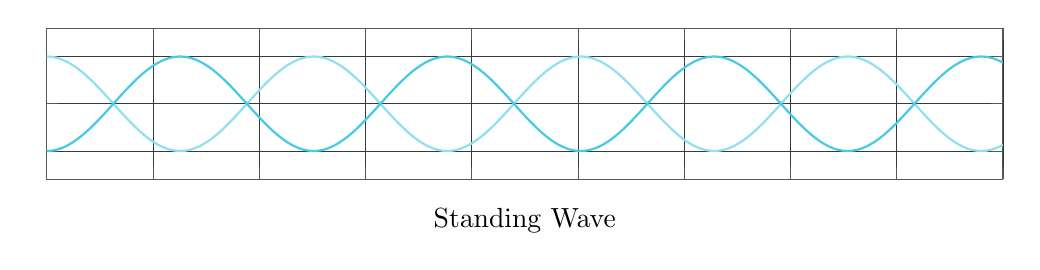
\begin{tikzpicture}
		\begin{axis}[
				height=3.5cm,
				width=\textwidth+1.6cm,
				domain=0:90,
				xmin=0,
				xmax=90,
				xlabel=Standing Wave,
				ytick={},
				yticklabels={},
				xtick={},
				xticklabels={},
				ymax=0.8,
				ymin=-0.8,
				ylabel={},
				grid=both,
				major grid style={line width=.2pt,draw=pag!95},
				samples=400,
				ylabel=,
				every axis/.append style={axis line style={pag!80}, tick style={pag!80}}
			]
			\addplot[p3, smooth, thick] {0.5*cos(deg((0.25*(x))))};
			\addplot[p4, smooth, thick] {0.5*cos(deg(0.25*(x-6.28*2)))};
		\end{axis}
	\end{tikzpicture}
\end{center}

There are a multitude of cases we will look at where a standing wave can occur, some with the same equations.

\textbf{Dual Fixed End String} - In this case, both ends of a string are fixed. The resonant frequncies occour when the wavelength is a multiple of half the length $L$.
\begin{center}
	\hspace*{-8pt}
	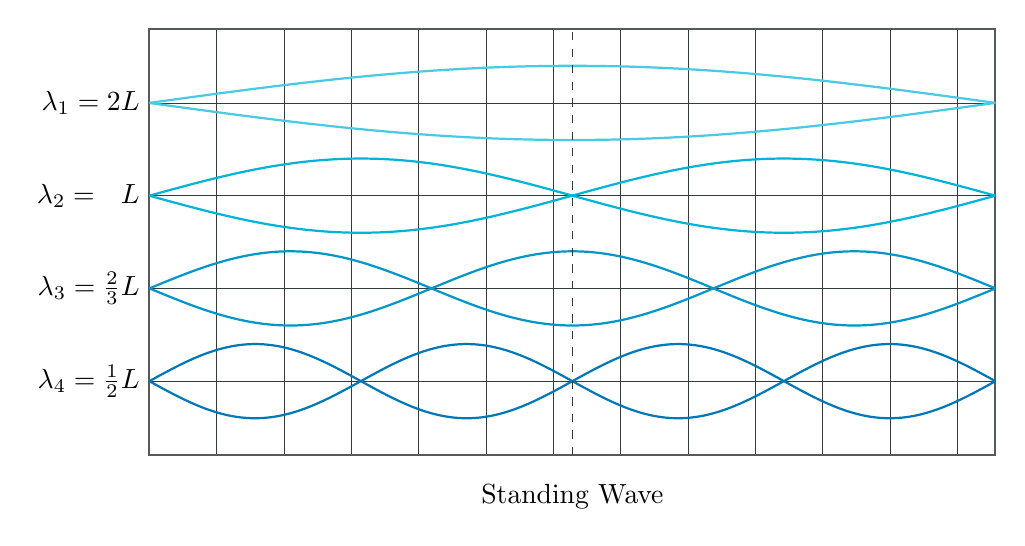
\begin{tikzpicture}
		\begin{axis}[
				height=7cm,
				width=\textwidth+0.2cm,
				domain=0:90,
				xmin=0,
				xmax=25.13,
				xlabel=Standing Wave,
				ytick={},
				yticklabels={
					$\lambda=2L$,
					$\lambda_4=\frac{1}{2}L$,
					$\lambda_3=\frac{2}{3}L$,
					$\lambda_2=\:\:\:L$,
					$\lambda_1=2L$
				},
				xtick={},
				xticklabels={},
				ymax=0.9,
				ymin=-1.4,
				ylabel={},
				grid=both,
				major grid style={line width=.2pt,draw=pag!95},
				samples=400,
				ylabel=,
				every axis/.append style={axis line style={pag!80, line width=0.75pt}, tick style={pag!95}}
			]
			\newcommand{\feat}{0.2}

			\addplot[p4, smooth, thick] {0.5+(\feat*sin(deg(0.125*((x)))))};
			\addplot[p4, smooth, thick] {0.5+(\feat*sin(deg(0.125*(x-3.14*8))))};

			\addplot[p5, smooth, thick] {0+(\feat*sin(deg(0.25*((x)))))};
			\addplot[p5, smooth, thick] {0+(\feat*sin(deg(0.25*(x-3.14*4))))};

			\addplot[p6, smooth, thick] {-0.5+(\feat*sin(deg((0.375*x)-9.42477)))};
			\addplot[p6, smooth, thick] {-0.5+(\feat*sin(deg((0.375*x))))};

			\addplot[p7, smooth, thick] {-1+(\feat*sin(deg((0.5*x)-3.14)))};
			\addplot[p7, smooth, thick] {-1+(\feat*sin(deg((0.5*x))))};

			\draw[dashed, color=pag!95] (axis cs:12.56,\pgfkeysvalueof{/pgfplots/ymin}) -- (axis cs:12.56,\pgfkeysvalueof{/pgfplots/ymax});

		\end{axis}
	\end{tikzpicture}
\end{center}

 In order for a standing wave to occur, we see we need certain wavelengths, which can be set by changing the frequency of the wave. The frequency number is the number nodes minus 1.

\begin{center}
	$f=\frac{v}{\lambda} \quad\ \longrightarrow \quad\ f_n=\frac{nv}{2L}=nf_1$\\
	\vspace{\baselineskip}
	$L=$ String Length $\:\:\:\:$ $v=$ Wave Speed $\:\:\:\:$ $n=$
	Frequency Number
\end{center}
\textbf{Fundamental Frequency} - The fundamental frequency is $f_1$, or the lowest frequency required for a standing wave to occur. It is also called the 1st harmonic. Subsequently, $f_2$ would be the 2nd harmonic.\\
\\
\\
\textbf{Special Case} - In all of these equations, it is impossible to determine the amplitude of the wave. We do deal with one special case, where two waves propagate in opposite directions on an infinite string. We can use the formula below to describe the resultant wave. The nodes in this wave are where amplitude is zero, or every half wavelength. \\
\begin{center}
	$y_{net}\left(x,t\right)=\underbrace{2A\sin\left(kx\right)}_{amplitude}\sin\left(\omega t\right)$
\end{center}
\vspace{\baselineskip}
\textbf{Dual Closed End Pipe} - The same equations can be used for sound waves in a pipe with both ends closed. In this case however, the vertical displacement is actually the horizontal displacement of each particle from there rest position. In this standing wave, there are nodes at each end of the pipe.
\begin{center}

	\hspace*{-8pt}	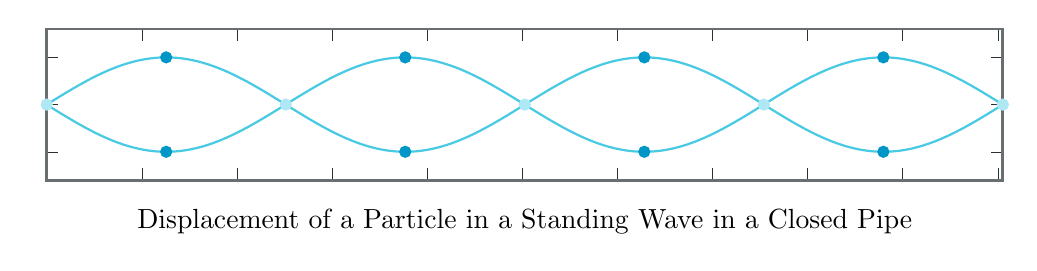
\begin{tikzpicture}
		\begin{axis}[
				height=3.5cm,
				width=\textwidth+1.6cm,
				domain=0:90,
				xmin=0,
				xmax=pi*16,
				xlabel=Displacement of a Particle in a Standing Wave in a Closed Pipe,
				ytick={},
				yticklabels={},
				xtick={},
				xticklabels={},
				ymax=0.8,
				ymin=-0.8,
				ylabel={},
				grid=none,
				samples=400,
				ylabel=,
				every axis/.append style={axis line style={pag!70,line width=1pt}, tick style={pag}}
			]
			\addplot[p4, smooth, thick] {0.5*sin(deg((0.25*(x))};
			\addplot[p4, smooth, thick] {0.5*sin(deg(0.25*(x-6.28*2))};
			\addplot[mark=*, p2, only marks] coordinates {(0,0) (pi*4,0) (pi*8,0) (pi*12,0) (pi*16,0)};
			\addplot[mark=*, p6, only marks] coordinates {(pi*2,-0.5) (pi*6,-0.5) (pi*10,-0.5) (pi*14,-0.5) (pi*2,0.5) (pi*6,0.5) (pi*10,0.5) (pi*14,0.5)};

		\end{axis}
	\end{tikzpicture}
\end{center}
\vspace{\baselineskip}
\textbf{Dual Open Ended Pipe} - This is the same as the previous, but the ends are actually anti-nodes. All the nodes and
\begin{center}

	\hspace*{-8pt}	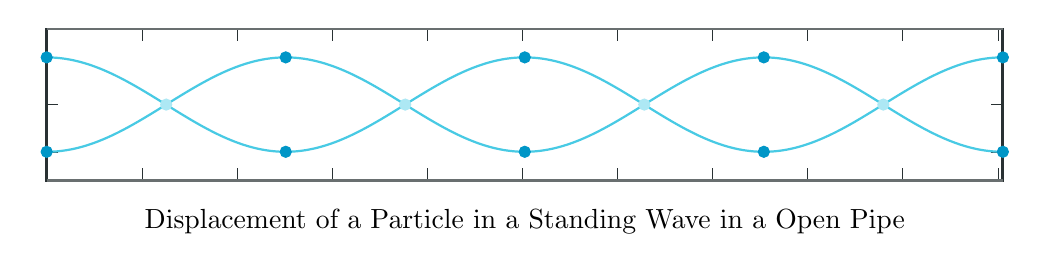
\begin{tikzpicture}
		\begin{axis}[
				height=3.5cm,
				width=\textwidth+1.6cm,
				domain=0:pi*16,
				xmin=0,
				xmax=pi*16,
				xlabel=Displacement of a Particle in a Standing Wave in a Open Pipe,
				ytick={},
				yticklabels={},
				xtick={},
				xticklabels={},
				ymax=0.8,
				ymin=-0.8,
				ylabel={},
				grid=none,
				samples=400,
				ylabel=,
				clip=false,
				every axis/.append style={axis line style={pag,line width=1pt}, tick style={pag}},
			]
			\addplot[pag!70, line width=1pt] coordinates {(0,0.8) (16*pi,0.8)};
			\addplot[pag!70, line width=1pt] coordinates {(0,-0.8) (16*pi,-0.8)};
			\addplot[p4, smooth, thick] {0.5*sin(deg((0.25*(x-6.28*3))};
			\addplot[p4, smooth, thick] {0.5*sin(deg(0.25*(x-6.28))};
			\addplot[mark=*, p2, only marks] coordinates {(pi*2,0) (pi*6,0) (pi*10,0) (pi*14,0)};
			\addplot[mark=*, p6, only marks] coordinates {(0,-0.5) (pi*4,-0.5) (pi*8,-0.5) (pi*12,-0.5) (pi*16,-0.5) (0,0.5) (pi*4,0.5) (pi*8,0.5) (pi*12,0.5) (pi*16,0.5)};

		\end{axis}

	\end{tikzpicture}
\end{center}
\vspace{\baselineskip}
In both these examples, the pressure wave graph has nodes opposite of the displacement wave graph. Recall that the pressure wave is out of phase with the displacement wave.
\vspace{-2pt}
\begin{center}
	
\begin{tikzpicture}
		\draw[fill=p2, color=p6] (0,0) circle [radius=0.1];
		\node at (3.5,0) {Displacement Node / Pressure Anti-node};
		\draw[fill=p6, color=p2] (8,0) circle [radius=0.1];
		\node at (11.5,0) {Displacement Anti-node / Pressure Node};
	\end{tikzpicture}
\end{center}
\vspace{\baselineskip}
\textbf{Single Closed End Pipe} - For an pipe with only one side closed, the formula changes. This time, in a standing wave, an anti-node always occurs at the open end, while a node occurs at the closed end.
\begin{center}

	\hspace*{-8pt}
	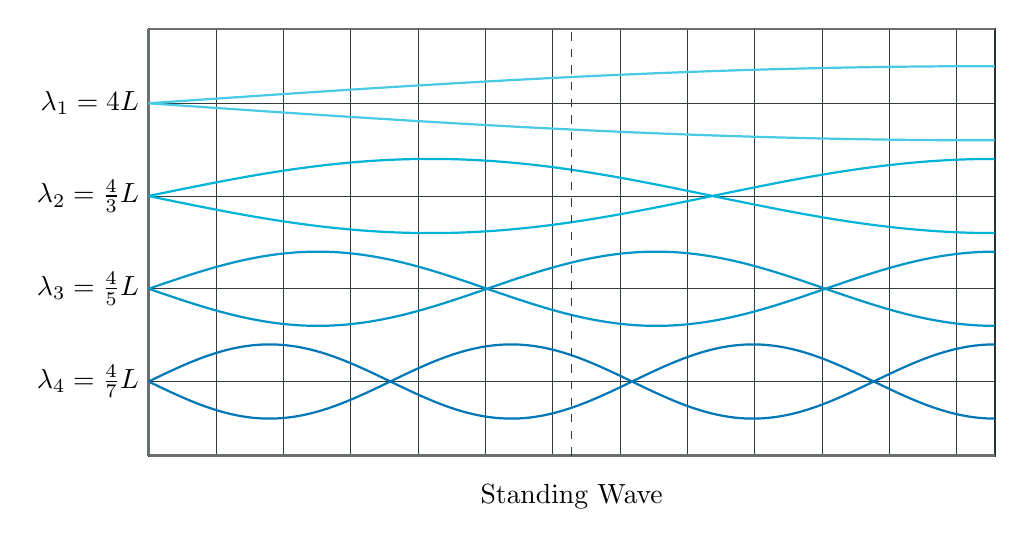
\begin{tikzpicture}
		\begin{axis}[
				height=7cm,
				width=\textwidth+0.2cm,
				domain=0:25.13,
				xmin=0,
				xmax=25.13,
				xlabel=Standing Wave,
				ytick={},
				yticklabels={$\lambda=2L$,$\lambda_4=\frac{4}{7}L$,$\lambda_3=\frac{4}{5}L$,$\lambda_2=\frac{4}{3}L$,$\lambda_1=4L$},
				xtick={},
				xticklabels={},
				ymax=0.9,
				ymin=-1.4,
				ylabel={},
				grid=both,
				major grid style={line width=.2pt,draw=pag!95},
				samples=400,
				ylabel=,
				clip=false,
				every axis/.append style={axis line style={pag, line width=0.75pt}, tick style={pag!95}}
			]
			\addplot[pag!70, line width=1pt] coordinates {(0,0.9) (25.13,0.9)};
			\addplot[pag!70, line width=1pt] coordinates {(0,-1.4) (25.13,-1.4)};
			\addplot[pag!70, line width=1pt] coordinates {(0,0.9) (0,-1.4)};
			\newcommand{\feat}{0.2}
			\addplot[p4, smooth, thick] {0.5+(\feat*sin(deg(0.0625*((x)))};
			\addplot[p4, smooth, thick] {0.5+(\feat*sin(deg(0.0625*(x-3.14*16)))};

			\addplot[p5, smooth, thick] {0+(\feat*sin(deg(0.1875*((x)))};
			\addplot[p5, smooth, thick] {0+(\feat*sin(deg(0.1875*(x-3.14*5.33333)))};

			\addplot[p6, smooth, thick] {-0.5+(\feat*sin(deg((0.3125*x)-9.42477))))};

			\addplot[p6, smooth, thick] {-0.5+(\feat*sin(deg((0.3125*x)))))};
			\

			\addplot[p7, smooth, thick] {-1+(\feat*sin(deg((0.4375*x)-3.14))))};

			\addplot[p7, smooth, thick] {-1+(\feat*sin(deg((0.4375*x)))))};

			\draw[dashed, color=pag!95] (axis cs:12.56,\pgfkeysvalueof{/pgfplots/ymin}) -- (axis cs:12.56,\pgfkeysvalueof{/pgfplots/ymax});

		\end{axis}
	\end{tikzpicture}
\end{center}
Again, these resonant frequencies only occour at certain wavelengths. The formula this time is similar, however, $n$ can only be \textbf{odd} numbers. To account for this, we append the formula to associate each $n$ with an odd number.
\begin{center}
	$f_n=\frac{\left(2n-1\right)v}{4L} \:\:\:\:\: f_n\neq nf_1$

	\vspace{\baselineskip}
	$L=$ String Length $\:\:\:\:$ $v=$ Wave Speed $\:\:\:\:$ $n=$
	Frequency Number
\end{center}
\vspace{\baselineskip}
\textbf{Waves in Music} - In music, there are two main catagories of instruments that produce waves. Stringed and wind.\\
\begin{adjustwidth}{1cm}{0cm}
	Stringed Instruments - A force is applied to a string. When the force is applied, a number different frequencies are propagated down the string, however, they quickly cancel themselves out leaving only the resonant frequencies.\\
	\\
	Wind Instruments - In wind instruments, the standing wave that occours is that of the resonant frequencies of the tube.
\end{adjustwidth}
\vspace{20pt}

\textbf{Optics} - Optics is the study of light and its behaviors. We often talk about image production and the ways we can make them.\\
\\
\begin{figure}[h]

	\begin{minipage}{0.62\textwidth}
		\textbf{Reflection} - The first thing we need to define is reflection. Recall that the angle of the incident ray from the normal (center) is the same as the reflected ray or rather $\theta_i=\theta_f$. This applies only for flat mirrors.

	\end{minipage}
	\begin{minipage}{0.3\textwidth}
		\hspace{5pt}	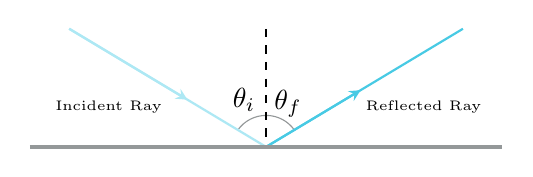
\begin{tikzpicture}
			\draw[pag!50] (0,0.4) arc (90:145:0.44);
			\draw[pag!50] (0,0.4) arc (90:35:0.44);

			\draw[p2,thick] (-2.5,1.5) -- (0,0);
			\draw[p2,thick,-{stealth[length=3mm]}] (-2.5,1.5) -- (-1,0.6);

			\draw[p4,thick] (2.5,1.5) -- (0,0);
			\draw[p4,thick,-{stealth[length=3mm]}] (0,0) -- (1.2,0.72);

			\draw[thick, dashed] (0,1.5) -- (0,0);
			\node at (-0.28,0.6) {$\theta_i$};
			\node at (0.28,0.55) {$\theta_f$};
			\node at (-2,0.5) {\tiny Incident Ray};
			\node at (2,0.5) {\tiny Reflected Ray};

			\draw[ultra thick, pag!50] (-3,0) -- (3,0);
		\end{tikzpicture}

	\end{minipage}

\end{figure}

\begin{figure}[h]

	\begin{minipage}{0.62\textwidth}
		\textbf{Flat Mirror} - We can illustrate the resultant image from a flat mirror using ray tracing. In this diagram, the image is virtual, meaning we perceive the rays as coming from behind the mirror. Each reflected ray can be traced back into the mirror, forming a virtual image of the object.
	\end{minipage}
	\begin{minipage}{0.2\textwidth}
		\hspace*{5pt}	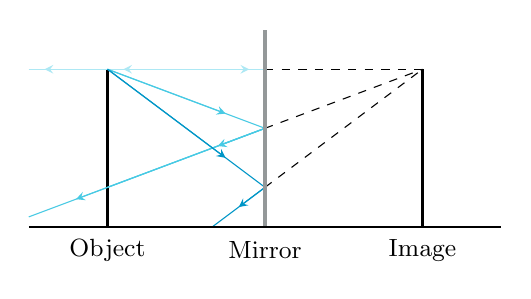
\begin{tikzpicture}

			% Object line
			\draw[thick] (-2,0) -- (-2,2);

			% Image Line
			\draw[thick] (2,0) -- (2,2);

			% Ray 1
			\draw[p2] (-3,2) -- (0,2);
			\draw[p2,{stealth[length=3mm]}-] (-1.8,2) -- (-0.5,2);
			\draw[p2,-{stealth[length=3mm]}] (-1,2) -- (-0.2,2);
			\draw[p2,{stealth[length=3mm]}-,color=p2] (-2.8,2) -- (-0.2,2);
			\draw[dashed] (0,2) -- (2,2);

			\draw[color=p2] (-3,2) -- (0,2);

			% Ray 2	
			\draw[p4,] (-2,2) -- (0,1.25);
			\draw[p4,-{stealth[length=3mm]}] (-2,2) -- (-0.5,1.4375);
			\draw[p4,] (0,1.25) -- (-2,0.5);
			\draw[p4,] (0,1.25) -- (-3,0.125);
			\draw[p4,-{stealth[length=3mm]}] (0,1.25) -- (-0.6,1.025);
			\draw[p4,-{stealth[length=3mm]}] (0,1.25) -- (-2.4,0.35);
			\draw[dashed] (0,1.25) -- (2,2);

			% Ray 3
			\draw[p6,] (-2,2) -- (0,0.5);
			\draw[p6,-{stealth[length=3mm]}] (-2,2) -- (-0.5,(2-0.75*1.5);
			\draw[p6,] (0,0.5) -- (-0.66666666,0);
			\draw[p6,-{stealth[length=3mm]}] (0,0.5) -- (-0.333333,0.25);
			\draw[dashed] (0,0.5) -- (2,2);
			\node at (-2,-0.3) {\small Object};
			\node at (2,-0.3) {\small Image};
			\node at (0,-0.3) {\small Mirror};

			% Normal line
			\draw[ultra thick,pag!50] (0,0) -- (0,2.5);
			% Mirror line
			\draw[thick] (-3,0) -- (3,0);
		\end{tikzpicture}
	\end{minipage}

\end{figure}

\begin{figure}[h]

	\begin{minipage}{0.62\textwidth}
		\textbf{Sign Convention} - It is important to keep in mind the sign convention when we are dealing with images. When talking about mirrors, the horizontal distance is negative when we go past the mirror. In the diagram on the right, $n$ simply refers to some unit of length.
	\end{minipage}
	\begin{minipage}{0.2\textwidth}
		\hspace*{0pt}	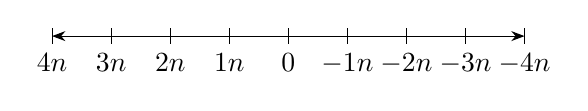
\begin{tikzpicture}
			% Draw the number line
			\draw[<->,>=Stealth] (-3,0) -- (3,0);

			\foreach \n/\label in {0/0,0.75/-1n,1.5/-2n,2.25/-3n,3/-4n,-0.75/1n,-1.5/2n,-2.25/3n,-3/4n} {
					\draw (\n,0.1) -- (\n,-0.1) node[below] {$\label$};
				}

		\end{tikzpicture}
	\end{minipage}

\end{figure}

\hspace{-15pt}\begin{minipage}{0.62\textwidth}
	\textbf{Magnification} - The magnification is simply the image height divided by the object height. A larger image means a greater magnification. Magnification is defined as $M=\frac{I}{O}=\frac{-v}{u}$. We can also define it using the horizontal distance of the image. A negative magnification is a inverted image. We add a negative into the formula because $v$ is negative by nature.
\end{minipage}
\begin{minipage}{0.2\textwidth}
	\hspace*{5pt}	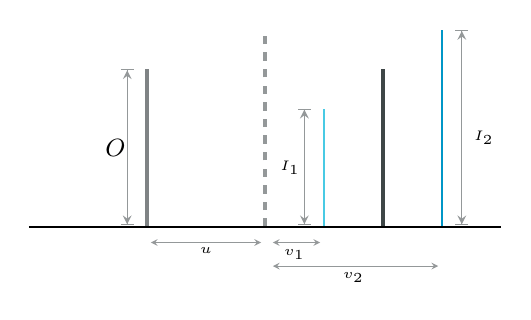
\begin{tikzpicture}

		% Object line
		\draw[ultra thick, pag!60] (-1.5,0) -- (-1.5,2);
		\draw[thin,|{stealth}-{stealth}|, pag!50] (-1.75,0.018) -- (-1.75,2);
		\node at (-1.9, 1) {\small $O$};

		% Image Line
		\draw[ultra thick, pag!90] (1.5,0) -- (1.5,2);

		% Image Line
		\draw[thick, p4] (0.75,0) -- (0.75,1.5);
		\draw[thin,|{stealth}-{stealth}|, pag!50] (0.5,0.018) -- (0.5,1.5);
		\node at (0.32, 0.75) {\tiny $I_1$};

		\draw[thick, p6] (2.25,0) -- (2.25,2.5);
		\draw[thin,|{stealth}-{stealth}|, pag!50] (2.5,0.018) -- (2.5,2.5);
		\node at (2.78, 1.125) {\tiny $I_2$};

		% Normal line
		\draw[ultra thick,pag!50, dashed] (0,0) -- (0,2.5);
		% Mirror line
		\draw[thick] (-3,0) -- (3,0);

		\draw[ultra thin,{stealth}-{stealth}, pag!50] (-1.45,-0.2) -- (-0.05,-0.2);
		\draw[ultra thin,{stealth}-{stealth}, pag!50] (0.1,-0.2) -- (0.7,-0.2);
		\draw[ultra thin,{stealth}-{stealth}, pag!50] (0.1,-0.5) -- (2.2,-0.5);
		\node at (-0.75, -0.3) {\tiny $u$};
		\node at (0.375, -0.35) {\tiny $v_1$};
		\node at (1.125, -0.65) {\tiny $v_2$};

	\end{tikzpicture}
\end{minipage}

\hspace{-15pt}\begin{minipage}{0.62\textwidth}
	\textbf{Concave Spherical Mirrors} - When dealing with spherical mirrors, we the center point ($C$) defines the radius of the arc derived from the mirror. The central axis is the line centered with the mirror, or the dashed line on the right. When a ray of light hits mirror parallel to the central axis, it's reflection passes through the focal point, or the \textit{real focus}, $F$. The focus point is half the radius, or rather $F=\frac{1}{2}\cdot C$. The center point is also called the center of curvature, while its magnitude is called the radius of curvature.
\end{minipage}
\begin{minipage}{0.2\textwidth}
	\hspace*{5pt}		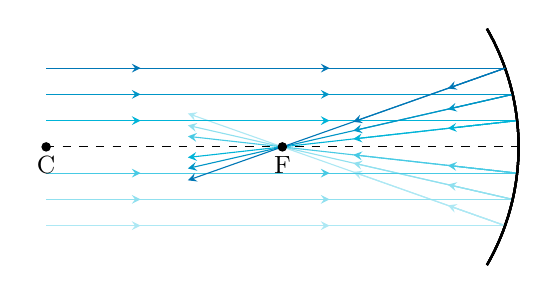
\begin{tikzpicture}

		% Draw the concave mirror
		\newcommand{\circdeg}{30}
		\newcommand{\rcirc}{3}
		\newcommand{\rlength}{6}
		\newcommand{\rayqx}{1.8}
		\newcommand{\concaveonec}{pag!50}
		% Draw the central axis
		\draw[dashed] (0,0) -- (\rlength,0);

		\newcommand{\drawLines}[2]{ % #1 represents the value for \rayqy, #2 for shade number
		\draw[thick] ({\rlength-(\rcirc-(\rcirc*cos((\circdeg))))},{0-(((sin(\circdeg))*\rcirc))}) arc (-\circdeg:\circdeg:\rcirc);

		\draw[color=p#2] (0,#1) -- ({\rlength- (\rcirc- ( ( ((\rcirc)^2) - ((#1)^2) )^(0.5) ))},#1);
		\draw[color=p#2,-{stealth}] (0,#1) -- (\rlength*0.6,#1);
		\draw[color=p#2,-{stealth}] (0,#1) -- (\rlength*0.2,#1);

		\draw[-{stealth},color=p#2] ({\rlength- (\rcirc- ( ( ((\rcirc)^2) - ((#1)^2) )^(0.5) ))},#1) -- (\rayqx,{( \rayqx-(\rlength/2))*(#1/( (\rlength/2)-(\rcirc- ( ( ((\rcirc)^2) - ((#1)^2) )^(0.5) ))   )});

		\draw[-{stealth},color=p#2] ({\rlength- (\rcirc- ( ( ((\rcirc)^2) - ((#1)^2) )^(0.5) ))},#1) -- ({\rlength*0.65},{( (\rlength*0.65)-(\rlength/2))*(#1/( (\rlength/2)-(\rcirc- ( ( ((\rcirc)^2) - ((#1)^2) )^(0.5) ))   )});

		\draw[-{stealth},color=p#2] ({\rlength- (\rcirc- ( ( ((\rcirc)^2) - ((#1)^2) )^(0.5) ))},#1) -- ({(\rlength*0.85)},{( (\rlength*0.85)-(\rlength/2))*(#1/( (\rlength/2)-(\rcirc- ( ( ((\rcirc)^2) - ((#1)^2) )^(0.5) ))   )});
		}

		\newcounter{shadeCounter}
		\setcounter{shadeCounter}{2} % Initialize the counter to 1 (for the first shade)

		\foreach \rayqy in {-1,{-2/3},{-1/3},{1/3},{2/3},1}{
				\drawLines{\rayqy}{\theshadeCounter} % Use the current value of the counter for the shade
				\addtocounter{shadeCounter}{1} % Increment the counter by 2 for the next shade
			}

		% Mark the focus point (halfway between mirror and center)
		\filldraw (\rlength/2,0) circle (1.5pt) node[below] {\small F};

		% Mark the center point (center of the mirror)
		\filldraw (0,0) circle (1.5pt) node[below] {\small C};

		% Optional: Add rays (incident and reflected)
		% \draw[->] (3,0.5) -- (1,0);  % Example of an incident ray
		% \draw[->] (1,0) -- (3,-0.5); % Example of a reflected ray
	\end{tikzpicture}

\end{minipage}

\hspace{-15pt}\begin{minipage}{0.62\textwidth}
	\textbf{Convex Spherical Mirrors} - Dealing with convex circular mirrors is relatively simple. Any line that strikes the mirror parallel with the central axis will be reflected about the line made from the point of striking the mirror, to the focus, which is negative. The focal point is negative, since it is on the opposite side of the mirror, or rather, virtual.
\end{minipage}
\begin{minipage}{0.2\textwidth}
	\hspace*{12pt}			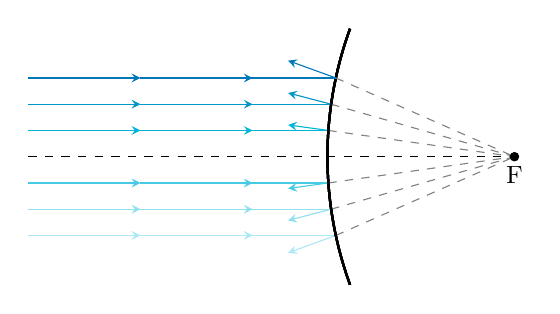
\begin{tikzpicture}

		% Draw the concave mirror
		\newcommand{\circdeg}{20}
		\newcommand{\rcircc}{-4.75}
		\newcommand{\rlength}{-\rcircc}
		\newcommand{\rayqx}{2}
		\newcommand{\concaveonec}{pag!50}
		\newcommand{\temptempha}{0.5}
		% Draw the central axis
		\draw[dashed] (\rlength*0.2,0) -- (\rlength*1.5,0);

		\newcommand{\drawLines}[2]{ % #1 represents the value for \rayqy, #2 for shade number
		\draw[thick] ({\rlength-(\rcircc-(\rcircc*cos((\circdeg))))},{0-(((sin(\circdeg))*\rcircc))}) arc (-\circdeg:\circdeg:\rcircc);

		\draw[color=p#2] (\rlength/2,#1) -- ({\rlength- (\rcircc+ ( ( ((\rcircc)^2) - ((#1)^2) )^(0.5) ))},#1);
		\draw[color=p#2,-{stealth}] (\rlength/2,#1) -- (\rlength*0.8,#1);
		\draw[color=p#2,{stealth}-] (\rlength/2,#1) -- (\rlength*0.2,#1);

		\draw[pag!60, dashed, thin] ({\rlength- (\rcircc+ ( ( ((\rcircc)^2) - ((#1)^2) )^(0.5) ))},#1) -- ({\rlength+(\rlength/2)},0);

		\draw[color=p#2, -{stealth}] ({\rlength- (\rcircc+ ( ( ((\rcircc)^2) - ((#1)^2) )^(0.5) ))},#1) -- ({\rlength-\temptempha}, { #1+((\temptempha)*((#1)/ ((\rlength+(\rlength/2))-(\rlength- (\rcircc+ ( ( ((\rcircc)^2) - ((#1)^2) )^(0.5) ))) )))});

		}

		\newcounter{shadeCounterd}
		\setcounter{shadeCounterd}{2} % Initialize the counter to 1 (for the first shade)

		\foreach \rayqy in {-1,{-2/3},{-1/3},{1/3},{2/3},1}{
				\drawLines{\rayqy}{\theshadeCounterd} % Use the current value of the counter for the shade
				\addtocounter{shadeCounterd}{1} % Increment the counter by 2 for the next shade
			}

		% Mark the focus point (halfway between mirror and center)
		\filldraw ({\rlength+\rlength/2},0) circle (1.5pt) node[below] {\small F};

		% Mark the center point (center of the mirror)

		% Optional: Add rays (incident and reflected)
		% \draw[->] (3,0.5) -- (1,0);  % Example of an incident ray
		% \draw[->] (1,0) -- (3,-0.5); % Example of a reflected ray
	\end{tikzpicture}
\end{minipage}

\hspace{-15pt}\begin{minipage}{0.62\textwidth}
	\textbf{Spherical Aberration} - It is very important to note that while for the scope of this course we say that a reflected ray always passes through the focal point, in reality, spherical aberration occurs resulting in the diagram on the right. More specifically, we use paraxial approximation. The closer a ray is to the central axis, the less its reflection strays from the focal point. Paraxial approximation uses this assuming that the mirror is small relative to the radius of curvature, and subsequently that all the rays will pass through the real focus.
\end{minipage}
% Spherical Abberation Diagram
\begin{minipage}{0.2\textwidth}
	\vspace{-10pt}
	\hspace*{5pt}		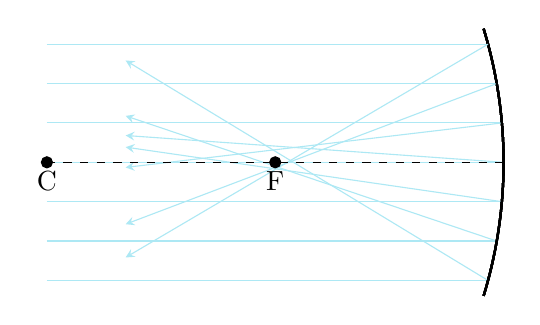
\begin{tikzpicture}
		% Draw the concave mirror
		\newcommand{\circdeg}{17}
		\newcommand{\rcirc}{5.8}
		\newcommand{\rlength}{5.8}
		\newcommand{\rayqx}{1}
		\newcommand{\concaveonec}{pag!50}

		\newcommand{\drawLines}[2]{ % #1 represents the value for \rayqy, #2 for shade number
		\draw[thick] ({\rlength-(\rcirc-(\rcirc*cos((\circdeg))))},{0-(((sin(\circdeg))*\rcirc))}) arc (-\circdeg:\circdeg:\rcirc);

		\draw[color=p#2] (0,#1) -- ({\rlength- (\rcirc- ( ( ((\rcirc)^2) - ((#1)^2) )^(0.5) ))},#1);

		\pgfmathsetmacro{\randomComponent}{(\rayqx-(\rlength/2))*(#1/( (\rlength/2)-(\rcirc- ( ( ((\rcirc)^2) - ((#1)^2) )^(0.5) ))) + rand*0.2}
		\draw[-{stealth},color=p#2] ({\rlength- (\rcirc- ( ( ((\rcirc)^2) - ((#1)^2) )^(0.5) ))},#1) -- (\rayqx,{\randomComponent});

		}

		\newcounter{shadeCounterw}
		\setcounter{shadeCounterw}{2} % Initialize the counter to 1 (for the first shade)

		\foreach \rayqy in {-1.5,-1,...,1.5}{
				\drawLines{\rayqy}{\theshadeCounterw} % Use the current value of the counter for the shade
				\addtocounter{shadeCounterw}{0} % Increment the counter by 2 for the next shade
			}

		% Draw the central axis
		\draw[dashed] (0,0) -- (\rlength,0);

		% Mark the focus point (halfway between mirror and center)
		\filldraw (\rlength/2,0) circle (2pt) node[below] {F};

		% Mark the center point (center of the mirror)
		\filldraw (0,0) circle (2pt) node[below] {C};

		% Optional: Add rays (incident and reflected)
		% \draw[->] (3,0.5) -- (1,0);  % Example of an incident ray
		% \draw[->] (1,0) -- (3,-0.5); % Example of a reflected ray
	\end{tikzpicture}

\end{minipage}
\vspace{20pt}

% Concave Spherical Mirror

\hspace{-16pt}
\begin{minipage}{16.5726cm}
	\textbf{Concave Ray Diagrams} - When drawing ray diagrams for concave mirrors, draw 4 general rays, when you can. First, parallel to the central axis. Second, to the central axis at the mirror. Third, draw through the focus. Fourth, draw through the central axis. An object beyond the focus produces a virtual image.
	\vspace{10pt}
\end{minipage}

% Diagram Varaibles

\newcommand{\dheight}{2.5}
\newcommand{\dwidth}{-10}
\newcommand{\dcircdeg}{7}
\newcommand{\rbcolor}{pag!70}
\newcommand{\rbocolor}{pag!97.5}
\newcommand{\scalecontrol}{0.5}
\newcommand{\imagethickness}{1.4pt}
\newcommand{\imagecolor}{pag!40}
\newcommand{\rcirc}{25}
\newcommand{\dspace}{15pt}
\newcommand{\newcolord}{!85!pag}
\newcommand{\tempscaler}{2.12}
\newcommand{\tempdistance}{90pt}

% Concave Mirror examples	

\hspace{-20pt}
\begin{minipage}{0.32\textwidth} % Diagram 1
	\fcolorbox{\rbcolor}{\rbocolor}{\begin{tikzpicture}[yscale=\scalecontrol, xscale={(16.5726/\tempscaler)/(abs(\dwidth)+\rcirc)}]
			\clip (\dwidth,-\dheight) rectangle (\rcirc,\dheight);
			% Draw the concave mirror
			\newcommand{\circdeg}{\dcircdeg}
			\newcommand{\rlength}{\rcirc}
			\newcommand{\rayqx}{\dwidth}
			\newcommand{\imaged}{-9}
			\newcommand{\height}{1.5}

			% Draw Object
			\draw [ultra thick] (\imaged,0) -- (\imaged,\height);
			% Calculate Image Distance
			\pgfmathsetmacro{\imagedis}{(\rlength-abs(  ( (2/\rlength)-(1/(\rcirc-\imaged))  )^(-1)   ))}
			% Calculate Image Height
			\pgfmathsetmacro{\imagehei}{\height* ((abs(((2/\rlength)-(1/(\rcirc-\imaged)))^(-1))) / (\rcirc-\imaged))  }
			% Draw Image
			\draw[line width=\imagethickness, \imagecolor] (\imagedis,0) -- (\imagedis, -\imagehei);
			% Draw the central axis
			\draw[dashed] (\rayqx,0) -- (\rlength,0);

			\newcommand{\parline}[2]{ % #1 represents the value for \rayqy, #2 for shade number
			\draw[thick] ({\rlength-(\rcirc-(\rcirc*cos((\circdeg))))},{0-(((sin(\circdeg))*\rcirc))}) arc (-\circdeg:\circdeg:\rcirc);

			\draw[color=p#2\newcolord] (\imaged,#1) -- ({\rlength- (\rcirc- ( ( ((\rcirc)^2) - ((#1)^2) )^(0.5) ))},#1);

			\draw[-{stealth},color=p#2\newcolord] ({\rlength- (\rcirc- ( ( ((\rcirc)^2) - ((#1)^2) )^(0.5) ))},#1) -- (\rayqx,{( \rayqx-(\rlength/2))*(#1/( (\rlength/2)-(\rcirc- ( ( ((\rcirc)^2) - ((#1)^2) )^(0.5) ))   )});}

			\newcommand{\drawLinez}[2]{ % #1 represents the value for \rayqy, #2 for shade number
			\draw[p#2\newcolord] (\imaged,#1) -- (\rlength,0);
			\draw[p#2\newcolord,-{stealth}] (\rlength,0) -- (\rayqx, {(0+ (\rayqx-\rlength)*( (#1) / ((\rlength-\imaged)   )  }  );}

			\newcommand{\drawLinezz}[2]{ % #1 represents the value for \rayqy, #2 for shade number
				\draw [{stealth}-,p#2\newcolord] (\rayqx, {0+(\rayqx * ( (#1)/(\imaged) ))}) -- ({\rcirc*( cos(atan((#1)/ (\imaged)))) }, {( ((\rcirc)^2) - ((\rcirc*( cos(atan((#1)/ (\imaged)))) )^2) )^(1/2) });}

			\newcommand{\drawRayThroughF}[2]{ % #1 represents the value for \rayqy
				% Define point F
				\pgfmathsetmacro{\xF}{\rlength/2}
				\pgfmathsetmacro{\yF}{0}

				% The top of the object line
				\pgfmathsetmacro{\xTop}{\imaged}
				\pgfmathsetmacro{\yTop}{#1}

				% Incident ray vector components from the top of the object to F
				\pgfmathsetmacro{\incidentX}{\xF - \xTop}
				\pgfmathsetmacro{\incidentY}{\yF - \yTop}

				% Normalize the incident ray vector
				\pgfmathsetmacro{\vecLength}{sqrt(\incidentX*\incidentX + \incidentY*\incidentY)}
				\pgfmathsetmacro{\dirX}{\incidentX/\vecLength}
				\pgfmathsetmacro{\dirY}{\incidentY/\vecLength}

				% Find the intersection with the mirror's arc by solving the system of equations 	parametrically
				% Circle's equation: x^2 + y^2 = rcirc^2
				% Parametric line equation: x = xTop + t*dirX, y = yTop + t*dirY
				\pgfmathsetmacro{\aQuad}{\dirX*\dirX + \dirY*\dirY}
				\pgfmathsetmacro{\bQuad}{2*\dirX*\xTop + 2*\dirY*\yTop}
				\pgfmathsetmacro{\cQuad}{\xTop*\xTop + \yTop*\yTop - \rcirc*\rcirc}
				\pgfmathsetmacro{\discriminant}{\bQuad*\bQuad - 4*\aQuad*\cQuad}

				% Since we know the ray must intersect the arc, we take the positive root for the 	parameter t
				\pgfmathsetmacro{\tValue}{(-\bQuad + sqrt(\discriminant)) / (2 * \aQuad)}

				% Calculate the intersection point
				\pgfmathsetmacro{\xIntersect}{\xTop + \tValue*\dirX}
				\pgfmathsetmacro{\yIntersect}{\yTop + \tValue*\dirY}

				% Draw the incident ray from the top of the object to the intersection point on the 	mirror arc
				\draw[p#2\newcolord, thick] (\xTop, \yTop) -- (\xIntersect, \yIntersect);
				\draw[p#2\newcolord, thick, -stealth] (\xIntersect, \yIntersect) -- (\rayqx, \yIntersect);}

			\parline{\height}{1}
			\drawLinez{\height}{3}
			\drawRayThroughF{\height}{7}

			% Mark the focus point (halfway between mirror and center)
			\filldraw (\rlength/2,0) circle (1.5pt) node[below] {\small F};

			% Mark the center point (center of the mirror)
			\filldraw (0,0) circle (1.5pt) node[below] {\small C};

		\end{tikzpicture}}
\end{minipage}
\hspace{\tempdistance}
\begin{minipage}{0.32\textwidth} % Diagram 2
	\fcolorbox{\rbcolor}{\rbocolor}{\begin{tikzpicture}[yscale=\scalecontrol, xscale={(16.5726/\tempscaler)/(abs(\dwidth)+\rcirc)}]
			\clip (\dwidth,-\dheight) rectangle (\rcirc,\dheight);
			% Draw the concave mirror
			\newcommand{\circdeg}{\dcircdeg}
			\newcommand{\rlength}{\rcirc}
			\newcommand{\rayqx}{\dwidth}
			\newcommand{\imaged}{-1.5}
			\newcommand{\height}{1.5}

			% Draw Object
			\draw [ultra thick] (\imaged,0) -- (\imaged,\height);
			% Calculate Image Distance
			\pgfmathsetmacro{\imagedis}{(\rlength-abs(  ( (2/\rlength)-(1/(\rcirc-\imaged))  )^(-1)   ))}
			% Calculate Image Height
			\pgfmathsetmacro{\imagehei}{\height* ((abs(((2/\rlength)-(1/(\rcirc-\imaged)))^(-1))) / (\rcirc-\imaged))  }
			% Draw Image
			\draw[line width=\imagethickness, \imagecolor] (\imagedis,0) -- (\imagedis, -\imagehei);
			% Draw the central axis
			\draw[dashed] (\rayqx,0) -- (\rlength,0);

			\newcommand{\parline}[2]{ % #1 represents the value for \rayqy, #2 for shade number
			\draw[thick] ({\rlength-(\rcirc-(\rcirc*cos((\circdeg))))},{0-(((sin(\circdeg))*\rcirc))}) arc (-\circdeg:\circdeg:\rcirc);

			\draw[color=p#2] (\imaged,#1) -- ({\rlength- (\rcirc- ( ( ((\rcirc)^2) - ((#1)^2) )^(0.5) ))},#1);

			\draw[-{stealth},color=p#2] ({\rlength- (\rcirc- ( ( ((\rcirc)^2) - ((#1)^2) )^(0.5) ))},#1) -- (\rayqx,{( \rayqx-(\rlength/2))*(#1/( (\rlength/2)-(\rcirc- ( ( ((\rcirc)^2) - ((#1)^2) )^(0.5) ))   )});}

			\newcommand{\drawLinez}[2]{ % #1 represents the value for \rayqy, #2 for shade number
			\draw[p#2] (\imaged,#1) -- (\rlength,0);
			\draw[p#2,-{stealth}] (\rlength,0) -- (\rayqx, {(0+ (\rayqx-\rlength)*( (#1) / ((\rlength-\imaged)   )  }  );}

			\newcommand{\drawLinezz}[2]{ % #1 represents the value for \rayqy, #2 for shade number
				\draw [{stealth}-,p#2] (\rayqx, {0+(\rayqx * ( (#1)/(\imaged) ))}) -- ({\rcirc*( cos(atan((#1)/ (\imaged)))) }, {( ((\rcirc)^2) - ((\rcirc*( cos(atan((#1)/ (\imaged)))) )^2) )^(1/2) });}

			\newcommand{\drawRayThroughF}[2]{ % #1 represents the value for \rayqy
				% Define point F
				\pgfmathsetmacro{\xF}{\rlength/2}
				\pgfmathsetmacro{\yF}{0}

				% The top of the object line
				\pgfmathsetmacro{\xTop}{\imaged}
				\pgfmathsetmacro{\yTop}{#1}

				% Incident ray vector components from the top of the object to F
				\pgfmathsetmacro{\incidentX}{\xF - \xTop}
				\pgfmathsetmacro{\incidentY}{\yF - \yTop}

				% Normalize the incident ray vector
				\pgfmathsetmacro{\vecLength}{sqrt(\incidentX*\incidentX + \incidentY*\incidentY)}
				\pgfmathsetmacro{\dirX}{\incidentX/\vecLength}
				\pgfmathsetmacro{\dirY}{\incidentY/\vecLength}

				% Find the intersection with the mirror's arc by solving the system of equations 	parametrically
				% Circle's equation: x^2 + y^2 = rcirc^2
				% Parametric line equation: x = xTop + t*dirX, y = yTop + t*dirY
				\pgfmathsetmacro{\aQuad}{\dirX*\dirX + \dirY*\dirY}
				\pgfmathsetmacro{\bQuad}{2*\dirX*\xTop + 2*\dirY*\yTop}
				\pgfmathsetmacro{\cQuad}{\xTop*\xTop + \yTop*\yTop - \rcirc*\rcirc}
				\pgfmathsetmacro{\discriminant}{\bQuad*\bQuad - 4*\aQuad*\cQuad}

				% Since we know the ray must intersect the arc, we take the positive root for the 	parameter t
				\pgfmathsetmacro{\tValue}{(-\bQuad + sqrt(\discriminant)) / (2 * \aQuad)}

				% Calculate the intersection point
				\pgfmathsetmacro{\xIntersect}{\xTop + \tValue*\dirX}
				\pgfmathsetmacro{\yIntersect}{\yTop + \tValue*\dirY}

				% Draw the incident ray from the top of the object to the intersection point on the 	mirror arc
				\draw[p#2, thick] (\xTop, \yTop) -- (\xIntersect, \yIntersect);
				\draw[p#2, thick, -stealth] (\xIntersect, \yIntersect) -- (\rayqx, \yIntersect);}

			\parline{\height}{1\newcolord}
			\drawLinez{\height}{3\newcolord}
			\drawRayThroughF{\height}{7\newcolord}

			% Mark the focus point (halfway between mirror and center)
			\filldraw (\rlength/2,0) circle (1.5pt) node[below] {\small F};

			% Mark the center point (center of the mirror)
			\filldraw (0,0) circle (1.5pt) node[below] {\small C};

		\end{tikzpicture}}
\end{minipage}

\vspace{\dspace}
\hspace{-20pt}
\begin{minipage}{0.32\textwidth} % Diagram 3
	\fcolorbox{\rbcolor}{\rbocolor}{\begin{tikzpicture}[yscale=\scalecontrol, xscale={(16.5726/\tempscaler)/(abs(\dwidth)+\rcirc)}]
			\clip (\dwidth,-\dheight) rectangle (\rcirc,\dheight);
			% Draw the concave mirror
			\newcommand{\circdeg}{\dcircdeg}
			\newcommand{\rlength}{\rcirc}
			\newcommand{\rayqx}{\dwidth}
			\newcommand{\imaged}{0}
			\newcommand{\height}{1.5}

			% Draw Object
			\draw [ultra thick] (\imaged,0) -- (\imaged,\height);
			% Calculate Image Distance
			\pgfmathsetmacro{\imagedis}{(\rlength-abs(  ( (2/\rlength)-(1/(\rcirc-\imaged))  )^(-1)   ))}
			% Calculate Image Height
			\pgfmathsetmacro{\imagehei}{\height* ((abs(((2/\rlength)-(1/(\rcirc-\imaged)))^(-1))) / (\rcirc-\imaged))  }
			% Draw Image
			\draw[line width=\imagethickness, \imagecolor] (\imagedis,0) -- (\imagedis, -\imagehei);
			% Draw the central axis
			\draw[dashed] (\rayqx,0) -- (\rlength,0);

			\newcommand{\parline}[2]{ % #1 represents the value for \rayqy, #2 for shade number
			\draw[thick] ({\rlength-(\rcirc-(\rcirc*cos((\circdeg))))},{0-(((sin(\circdeg))*\rcirc))}) arc (-\circdeg:\circdeg:\rcirc);

			\draw[color=p#2] (\imaged,#1) -- ({\rlength- (\rcirc- ( ( ((\rcirc)^2) - ((#1)^2) )^(0.5) ))},#1);

			\draw[-{stealth},color=p#2] ({\rlength- (\rcirc- ( ( ((\rcirc)^2) - ((#1)^2) )^(0.5) ))},#1) -- (\rayqx,{( \rayqx-(\rlength/2))*(#1/( (\rlength/2)-(\rcirc- ( ( ((\rcirc)^2) - ((#1)^2) )^(0.5) ))   )});}

			\newcommand{\drawLinez}[2]{ % #1 represents the value for \rayqy, #2 for shade number
			\draw[p#2] (\imaged,#1) -- (\rlength,0);
			\draw[p#2,-{stealth}] (\rlength,0) -- (\rayqx, {(0+ (\rayqx-\rlength)*( (#1) / ((\rlength-\imaged)   )  }  );}

			\newcommand{\drawLinezz}[2]{ % #1 represents the value for \rayqy, #2 for shade number
				\draw [{stealth}-,p#2] (\rayqx, {0+(\rayqx * ( (#1)/(\imaged) ))}) -- ({\rcirc*( cos(atan((#1)/ (\imaged)))) }, {( ((\rcirc)^2) - ((\rcirc*( cos(atan((#1)/ (\imaged)))) )^2) )^(1/2) });}

			\newcommand{\drawRayThroughF}[2]{ % #1 represents the value for \rayqy
				% Define point F
				\pgfmathsetmacro{\xF}{\rlength/2}
				\pgfmathsetmacro{\yF}{0}

				% The top of the object line
				\pgfmathsetmacro{\xTop}{\imaged}
				\pgfmathsetmacro{\yTop}{#1}

				% Incident ray vector components from the top of the object to F
				\pgfmathsetmacro{\incidentX}{\xF - \xTop}
				\pgfmathsetmacro{\incidentY}{\yF - \yTop}

				% Normalize the incident ray vector
				\pgfmathsetmacro{\vecLength}{sqrt(\incidentX*\incidentX + \incidentY*\incidentY)}
				\pgfmathsetmacro{\dirX}{\incidentX/\vecLength}
				\pgfmathsetmacro{\dirY}{\incidentY/\vecLength}

				% Find the intersection with the mirror's arc by solving the system of equations 	parametrically
				% Circle's equation: x^2 + y^2 = rcirc^2
				% Parametric line equation: x = xTop + t*dirX, y = yTop + t*dirY
				\pgfmathsetmacro{\aQuad}{\dirX*\dirX + \dirY*\dirY}
				\pgfmathsetmacro{\bQuad}{2*\dirX*\xTop + 2*\dirY*\yTop}
				\pgfmathsetmacro{\cQuad}{\xTop*\xTop + \yTop*\yTop - \rcirc*\rcirc}
				\pgfmathsetmacro{\discriminant}{\bQuad*\bQuad - 4*\aQuad*\cQuad}

				% Since we know the ray must intersect the arc, we take the positive root for the 	parameter t
				\pgfmathsetmacro{\tValue}{(-\bQuad + sqrt(\discriminant)) / (2 * \aQuad)}

				% Calculate the intersection point
				\pgfmathsetmacro{\xIntersect}{\xTop + \tValue*\dirX}
				\pgfmathsetmacro{\yIntersect}{\yTop + \tValue*\dirY}

				% Draw the incident ray from the top of the object to the intersection point on the 	mirror arc
				\draw[p#2, thick] (\xTop, \yTop) -- (\xIntersect, \yIntersect);
				\draw[p#2, thick, -stealth] (\xIntersect, \yIntersect) -- (\rayqx, \yIntersect);}

			\parline{\height}{1\newcolord}
			\drawLinez{\height}{3\newcolord}
			\drawRayThroughF{\height}{7\newcolord}

			% Mark the focus point (halfway between mirror and center)
			\filldraw (\rlength/2,0) circle (1.5pt) node[below] {\small F};

			% Mark the center point (center of the mirror)
			\filldraw (0,0) circle (1.5pt) node[below] {\small C};

		\end{tikzpicture}}
\end{minipage}
\hspace{\tempdistance}
\begin{minipage}{0.32\textwidth} % Diagram 4
	\fcolorbox{\rbcolor}{\rbocolor}{\begin{tikzpicture}[yscale=\scalecontrol, xscale={(16.5726/\tempscaler)/(abs(\dwidth)+\rcirc)}]
			\clip (\dwidth,-\dheight) rectangle (\rcirc,\dheight);
			% Draw the concave mirror
			\newcommand{\circdeg}{\dcircdeg}
			\newcommand{\rlength}{\rcirc}
			\newcommand{\rayqx}{\dwidth}
			\newcommand{\imaged}{1.5}
			\newcommand{\height}{1.5}

			% Draw Object
			\draw [ultra thick] (\imaged,0) -- (\imaged,\height);
			% Calculate Image Distance
			\pgfmathsetmacro{\imagedis}{(\rlength-abs(  ( (2/\rlength)-(1/(\rcirc-\imaged))  )^(-1)   ))}
			% Calculate Image Height
			\pgfmathsetmacro{\imagehei}{\height* ((abs(((2/\rlength)-(1/(\rcirc-\imaged)))^(-1))) / (\rcirc-\imaged))  }
			% Draw Image
			\draw[line width=\imagethickness, \imagecolor] (\imagedis,0) -- (\imagedis, -\imagehei);
			% Draw the central axis
			\draw[dashed] (\rayqx,0) -- (\rlength,0);

			\newcommand{\parline}[2]{ % #1 represents the value for \rayqy, #2 for shade number
			\draw[thick] ({\rlength-(\rcirc-(\rcirc*cos((\circdeg))))},{0-(((sin(\circdeg))*\rcirc))}) arc (-\circdeg:\circdeg:\rcirc);

			\draw[color=p#2] (\imaged,#1) -- ({\rlength- (\rcirc- ( ( ((\rcirc)^2) - ((#1)^2) )^(0.5) ))},#1);

			\draw[-{stealth},color=p#2] ({\rlength- (\rcirc- ( ( ((\rcirc)^2) - ((#1)^2) )^(0.5) ))},#1) -- (\rayqx,{( \rayqx-(\rlength/2))*(#1/( (\rlength/2)-(\rcirc- ( ( ((\rcirc)^2) - ((#1)^2) )^(0.5) ))   )});}

			\newcommand{\drawLinez}[2]{ % #1 represents the value for \rayqy, #2 for shade number
			\draw[p#2] (\imaged,#1) -- (\rlength,0);
			\draw[p#2,-{stealth}] (\rlength,0) -- (\rayqx, {(0+ (\rayqx-\rlength)*( (#1) / ((\rlength-\imaged)   )  }  );}

			\newcommand{\drawLinezz}[2]{ % #1 represents the value for \rayqy, #2 for shade number
				\draw [{stealth}-,p#2] (\rayqx, {0+(\rayqx * ( (#1)/(\imaged) ))}) -- ({\rcirc*( cos(atan((#1)/ (\imaged)))) }, {( ((\rcirc)^2) - ((\rcirc*( cos(atan((#1)/ (\imaged)))) )^2) )^(1/2) });}

			\newcommand{\drawRayThroughF}[2]{ % #1 represents the value for \rayqy
				% Define point F
				\pgfmathsetmacro{\xF}{\rlength/2}
				\pgfmathsetmacro{\yF}{0}

				% The top of the object line
				\pgfmathsetmacro{\xTop}{\imaged}
				\pgfmathsetmacro{\yTop}{#1}

				% Incident ray vector components from the top of the object to F
				\pgfmathsetmacro{\incidentX}{\xF - \xTop}
				\pgfmathsetmacro{\incidentY}{\yF - \yTop}

				% Normalize the incident ray vector
				\pgfmathsetmacro{\vecLength}{sqrt(\incidentX*\incidentX + \incidentY*\incidentY)}
				\pgfmathsetmacro{\dirX}{\incidentX/\vecLength}
				\pgfmathsetmacro{\dirY}{\incidentY/\vecLength}

				% Find the intersection with the mirror's arc by solving the system of equations 	parametrically
				% Circle's equation: x^2 + y^2 = rcirc^2
				% Parametric line equation: x = xTop + t*dirX, y = yTop + t*dirY
				\pgfmathsetmacro{\aQuad}{\dirX*\dirX + \dirY*\dirY}
				\pgfmathsetmacro{\bQuad}{2*\dirX*\xTop + 2*\dirY*\yTop}
				\pgfmathsetmacro{\cQuad}{\xTop*\xTop + \yTop*\yTop - \rcirc*\rcirc}
				\pgfmathsetmacro{\discriminant}{\bQuad*\bQuad - 4*\aQuad*\cQuad}

				% Since we know the ray must intersect the arc, we take the positive root for the 	parameter t
				\pgfmathsetmacro{\tValue}{(-\bQuad + sqrt(\discriminant)) / (2 * \aQuad)}

				% Calculate the intersection point
				\pgfmathsetmacro{\xIntersect}{\xTop + \tValue*\dirX}
				\pgfmathsetmacro{\yIntersect}{\yTop + \tValue*\dirY}

				% Draw the incident ray from the top of the object to the intersection point on the 	mirror arc
				\draw[p#2, thick] (\xTop, \yTop) -- (\xIntersect, \yIntersect);
				\draw[p#2, thick, -stealth] (\xIntersect, \yIntersect) -- (\rayqx, \yIntersect);}

			\parline{\height}{1\newcolord}
			\drawLinez{\height}{3\newcolord}
			\drawLinezz{\height}{5\newcolord}
			\drawRayThroughF{\height}{7\newcolord}

			% Mark the focus point (halfway between mirror and center)
			\filldraw (\rlength/2,0) circle (1.5pt) node[below] {\small F};

			% Mark the center point (center of the mirror)
			\filldraw (0,0) circle (1.5pt) node[below] {\small C};

		\end{tikzpicture}}
\end{minipage}

\vspace{\dspace}
\hspace{-20pt}
\begin{minipage}{0.32\textwidth} % Diagram 5
	\fcolorbox{\rbcolor}{\rbocolor}{\begin{tikzpicture}[yscale=\scalecontrol, xscale={(16.5726/\tempscaler)/(abs(\dwidth)+\rcirc)}]
			\clip (\dwidth,-\dheight) rectangle (\rcirc,\dheight);
			% Draw the concave mirror
			\newcommand{\circdeg}{\dcircdeg}
			\newcommand{\rlength}{\rcirc}
			\newcommand{\rayqx}{\dwidth}
			\newcommand{\imaged}{10}
			\newcommand{\height}{1.5}

			% Draw Object
			\draw [ultra thick] (\imaged,0) -- (\imaged,\height);
			% Calculate Image Distance
			\pgfmathsetmacro{\imagedis}{(\rlength-abs(  ( (2/\rlength)-(1/(\rcirc-\imaged))  )^(-1)   ))}
			% Calculate Image Height
			\pgfmathsetmacro{\imagehei}{\height* ((abs(((2/\rlength)-(1/(\rcirc-\imaged)))^(-1))) / (\rcirc-\imaged))  }
			% Draw Image
			\draw[line width=\imagethickness, \imagecolor] (\imagedis,0) -- (\imagedis, -\imagehei);
			% Draw the central axis
			\draw[dashed] (\rayqx,0) -- (\rlength,0);

			\newcommand{\parline}[2]{ % #1 represents the value for \rayqy, #2 for shade number
			\draw[thick] ({\rlength-(\rcirc-(\rcirc*cos((\circdeg))))},{0-(((sin(\circdeg))*\rcirc))}) arc (-\circdeg:\circdeg:\rcirc);

			\draw[color=p#2] (\imaged,#1) -- ({\rlength- (\rcirc- ( ( ((\rcirc)^2) - ((#1)^2) )^(0.5) ))},#1);

			\draw[-{stealth},color=p#2] ({\rlength- (\rcirc- ( ( ((\rcirc)^2) - ((#1)^2) )^(0.5) ))},#1) -- (\rayqx,{( \rayqx-(\rlength/2))*(#1/( (\rlength/2)-(\rcirc- ( ( ((\rcirc)^2) - ((#1)^2) )^(0.5) ))   )});}

			\newcommand{\drawLinez}[2]{ % #1 represents the value for \rayqy, #2 for shade number
			\draw[p#2] (\imaged,#1) -- (\rlength,0);
			\draw[p#2,-{stealth}] (\rlength,0) -- (\rayqx, {(0+ (\rayqx-\rlength)*( (#1) / ((\rlength-\imaged)   )  }  );}

			\newcommand{\drawLinezz}[2]{ % #1 represents the value for \rayqy, #2 for shade number
				\draw [{stealth}-,p#2] (\rayqx, {0+(\rayqx * ( (#1)/(\imaged) ))}) -- ({\rcirc*( cos(atan((#1)/ (\imaged)))) }, {( ((\rcirc)^2) - ((\rcirc*( cos(atan((#1)/ (\imaged)))) )^2) )^(1/2) });}

			\newcommand{\drawRayThroughF}[2]{ % #1 represents the value for \rayqy
				% Define point F
				\pgfmathsetmacro{\xF}{\rlength/2}
				\pgfmathsetmacro{\yF}{0}

				% The top of the object line
				\pgfmathsetmacro{\xTop}{\imaged}
				\pgfmathsetmacro{\yTop}{#1}

				% Incident ray vector components from the top of the object to F
				\pgfmathsetmacro{\incidentX}{\xF - \xTop}
				\pgfmathsetmacro{\incidentY}{\yF - \yTop}

				% Normalize the incident ray vector
				\pgfmathsetmacro{\vecLength}{sqrt(\incidentX*\incidentX + \incidentY*\incidentY)}
				\pgfmathsetmacro{\dirX}{\incidentX/\vecLength}
				\pgfmathsetmacro{\dirY}{\incidentY/\vecLength}

				% Find the intersection with the mirror's arc by solving the system of equations 	parametrically
				% Circle's equation: x^2 + y^2 = rcirc^2
				% Parametric line equation: x = xTop + t*dirX, y = yTop + t*dirY
				\pgfmathsetmacro{\aQuad}{\dirX*\dirX + \dirY*\dirY}
				\pgfmathsetmacro{\bQuad}{2*\dirX*\xTop + 2*\dirY*\yTop}
				\pgfmathsetmacro{\cQuad}{\xTop*\xTop + \yTop*\yTop - \rcirc*\rcirc}
				\pgfmathsetmacro{\discriminant}{\bQuad*\bQuad - 4*\aQuad*\cQuad}

				% Since we know the ray must intersect the arc, we take the positive root for the 	parameter t
				\pgfmathsetmacro{\tValue}{(-\bQuad + sqrt(\discriminant)) / (2 * \aQuad)}

				% Calculate the intersection point
				\pgfmathsetmacro{\xIntersect}{\xTop + \tValue*\dirX}
				\pgfmathsetmacro{\yIntersect}{\yTop + \tValue*\dirY}

				% Draw the incident ray from the top of the object to the intersection point on the 	mirror arc
				\draw[p#2, thick] (\xTop, \yTop) -- (\xIntersect, \yIntersect);
				\draw[p#2, thick, -stealth] (\xIntersect, \yIntersect) -- (\rayqx, \yIntersect);}

			\parline{\height}{1\newcolord}
			\drawLinez{\height}{3\newcolord}
			\drawLinezz{\height}{5\newcolord}
			\drawRayThroughF{\height}{7\newcolord}

			% Mark the focus point (halfway between mirror and center)
			\filldraw (\rlength/2,0) circle (1.5pt) node[below] {\small F};

			% Mark the center point (center of the mirror)
			\filldraw (0,0) circle (1.5pt) node[below] {\small C};

		\end{tikzpicture}}
\end{minipage}
\hspace{\tempdistance}
\begin{minipage}{0.32\textwidth} % Diagram 6
	\fcolorbox{\rbcolor}{\rbocolor}{\begin{tikzpicture}[yscale=\scalecontrol, xscale={(16.5726/\tempscaler)/(abs(\dwidth)+\rcirc)}]
			\clip (\dwidth,-\dheight) rectangle (\rcirc,\dheight);
			% Draw the concave mirror
			\newcommand{\circdeg}{\dcircdeg}
			\newcommand{\rlength}{\rcirc}
			\newcommand{\rayqx}{\dwidth}
			\newcommand{\imaged}{12.5}
			\newcommand{\height}{2}

			% Draw Object
			\draw [ultra thick] (\imaged,0) -- (\imaged,\height);
			% Draw the central axis
			\draw[dashed] (\rayqx,0) -- (\rlength,0);

			\newcommand{\parline}[2]{ % #1 represents the value for \rayqy, #2 for shade number
			\draw[thick] ({\rlength-(\rcirc-(\rcirc*cos((\circdeg))))},{0-(((sin(\circdeg))*\rcirc))}) arc (-\circdeg:\circdeg:\rcirc);

			\draw[color=p#2] (\imaged,#1) -- ({\rlength- (\rcirc- ( ( ((\rcirc)^2) - ((#1)^2) )^(0.5) ))},#1);

			\draw[-{stealth},color=p#2] ({\rlength- (\rcirc- ( ( ((\rcirc)^2) - ((#1)^2) )^(0.5) ))},#1) -- (\rayqx,{( \rayqx-(\rlength/2))*(#1/( (\rlength/2)-(\rcirc- ( ( ((\rcirc)^2) - ((#1)^2) )^(0.5) ))   )});}

			\newcommand{\drawLinez}[2]{ % #1 represents the value for \rayqy, #2 for shade number
			\draw[p#2] (\imaged,#1) -- (\rlength,0);
			\draw[p#2,-{stealth}] (\rlength,0) -- (\rayqx, {(0+ (\rayqx-\rlength)*( (#1) / ((\rlength-\imaged)   )  }  );}

			\newcommand{\drawLinezz}[2]{ % #1 represents the value for \rayqy, #2 for shade number
				\draw [{stealth}-,p#2] (\rayqx, {0+(\rayqx * ( (#1)/(\imaged) ))}) -- ({\rcirc*( cos(atan((#1)/ (\imaged)))) }, {( ((\rcirc)^2) - ((\rcirc*( cos(atan((#1)/ (\imaged)))) )^2) )^(1/2) });}

			\newcommand{\drawRayThroughF}[2]{ % #1 represents the value for \rayqy
				% Define point F
				\pgfmathsetmacro{\xF}{\rlength/2}
				\pgfmathsetmacro{\yF}{0}

				% The top of the object line
				\pgfmathsetmacro{\xTop}{\imaged}
				\pgfmathsetmacro{\yTop}{#1}

				% Incident ray vector components from the top of the object to F
				\pgfmathsetmacro{\incidentX}{\xF - \xTop}
				\pgfmathsetmacro{\incidentY}{\yF - \yTop}

				% Normalize the incident ray vector
				\pgfmathsetmacro{\vecLength}{sqrt(\incidentX*\incidentX + \incidentY*\incidentY)}
				\pgfmathsetmacro{\dirX}{\incidentX/\vecLength}
				\pgfmathsetmacro{\dirY}{\incidentY/\vecLength}

				% Find the intersection with the mirror's arc by solving the system of equations 	parametrically
				% Circle's equation: x^2 + y^2 = rcirc^2
				% Parametric line equation: x = xTop + t*dirX, y = yTop + t*dirY
				\pgfmathsetmacro{\aQuad}{\dirX*\dirX + \dirY*\dirY}
				\pgfmathsetmacro{\bQuad}{2*\dirX*\xTop + 2*\dirY*\yTop}
				\pgfmathsetmacro{\cQuad}{\xTop*\xTop + \yTop*\yTop - \rcirc*\rcirc}
				\pgfmathsetmacro{\discriminant}{\bQuad*\bQuad - 4*\aQuad*\cQuad}

				% Since we know the ray must intersect the arc, we take the positive root for the 	parameter t
				\pgfmathsetmacro{\tValue}{(-\bQuad + sqrt(\discriminant)) / (2 * \aQuad)}

				% Calculate the intersection point
				\pgfmathsetmacro{\xIntersect}{\xTop + \tValue*\dirX}
				\pgfmathsetmacro{\yIntersect}{\yTop + \tValue*\dirY}

				% Draw the incident ray from the top of the object to the intersection point on the 	mirror arc
				\draw[p#2, thick] (\xTop, \yTop) -- (\xIntersect, \yIntersect);
				\draw[p#2, thick, -stealth] (\xIntersect, \yIntersect) -- (\rayqx, \yIntersect);}

			\parline{\height}{1\newcolord}
			\drawLinez{\height}{3\newcolord}
			\drawLinezz{\height}{5\newcolord}

			% Mark the focus point (halfway between mirror and center)
			\filldraw (\rlength/2,0) circle (1.5pt) node[below] {\small F};

			% Mark the center point (center of the mirror)
			\filldraw (0,0) circle (1.5pt) node[below] {\small C};

		\end{tikzpicture}}
\end{minipage}

\vspace{10pt}
 The special concave case is below. The closer to the focus, the larger the image. The  image in this case is always virtual, and has a negative image distance
\vspace{5pt}

\hspace{-20pt}
\begin{minipage}{0.32\textwidth} % Diagram 6
	\fcolorbox{\rbcolor}{\rbocolor}{\begin{tikzpicture}[yscale=\scalecontrol, xscale={(16.5726/1.407)/(abs(\dwidth)+\rcirc)}]
			\clip (\dwidth,-\dheight) rectangle (\rcirc*1.56,\dheight);
			% Draw the concave mirror
			\newcommand{\circdeg}{\dcircdeg}
			\newcommand{\rlength}{25}
			\newcommand{\rayqx}{\dwidth}
			\newcommand{\imaged}{20}
			\newcommand{\height}{1.2}

			\draw[line width=\imagethickness, \imagecolor] (33.3333,2) -- (33.333,0);
			% Draw Object
			\draw [ultra thick] (\imaged,0) -- (\imaged,\height);
			% Draw the central axis
			\draw[dashed] (\rayqx,0) -- (\rlength+15,0);

			\newcommand{\parline}[2]{ % #1 represents the value for \rayqy, #2 for shade number
			\draw[thick] ({\rlength-(\rcirc-(\rcirc*cos((\circdeg))))},{0-(((sin(\circdeg))*\rcirc))}) arc (-\circdeg:\circdeg:\rcirc);

			\draw[color=p#2] (\imaged,#1) -- ({\rlength- (\rcirc- ( ( ((\rcirc)^2) - ((#1)^2) )^(0.5) ))},#1);

			\draw[-{stealth},color=p#2] ({\rlength-(\rcirc- ( ( ((\rcirc)^2) - ((#1)^2) )^(0.5) ))},#1) -- (\rayqx,{( \rayqx-(\rlength/2))*(#1/( (\rlength/2)-(\rcirc- ( ( ((\rcirc)^2) - ((#1)^2) )^(0.5) ))   )});}

			\newcommand{\drawLinez}[2]{ % #1 represents the value for \rayqy, #2 for shade number
			\draw[p#2] (\imaged,#1) -- (\rlength,0);
			\draw[p#2,-{stealth}] (\rlength,0) -- (\rayqx, {(0+ (\rayqx-\rlength)*( (#1) / ((\rlength-\imaged)   )  }  );}

			\newcommand{\drawLinezz}[2]{ % #1 represents the value for \rayqy, #2 for shade number
				\draw [{stealth}-,p#2] (\rayqx, {0+(\rayqx * ( (#1)/(\imaged) ))}) -- ({\rcirc*( cos(atan((#1)/ (\imaged)))) }, {( ((\rcirc)^2) - ((\rcirc*( cos(atan((#1)/ (\imaged)))) )^2) )^(1/2) });}

			\newcommand{\drawRayThroughF}[2]{ % #1 represents the value for \rayqy
				% Define point F
				\pgfmathsetmacro{\xF}{\rlength/2}
				\pgfmathsetmacro{\yF}{0}

				% The top of the object line
				\pgfmathsetmacro{\xTop}{\imaged}
				\pgfmathsetmacro{\yTop}{#1}

				% Incident ray vector components from the top of the object to F
				\pgfmathsetmacro{\incidentX}{\xF - \xTop}
				\pgfmathsetmacro{\incidentY}{\yF - \yTop}

				% Normalize the incident ray vector
				\pgfmathsetmacro{\vecLength}{sqrt(\incidentX*\incidentX + \incidentY*\incidentY)}
				\pgfmathsetmacro{\dirX}{\incidentX/\vecLength}
				\pgfmathsetmacro{\dirY}{\incidentY/\vecLength}

				% Find the intersection with the mirror's arc by solving the system of equations 	parametrically
				% Circle's equation: x^2 + y^2 = rcirc^2
				% Parametric line equation: x = xTop + t*dirX, y = yTop + t*dirY
				\pgfmathsetmacro{\aQuad}{\dirX*\dirX + \dirY*\dirY}
				\pgfmathsetmacro{\bQuad}{2*\dirX*\xTop + 2*\dirY*\yTop}
				\pgfmathsetmacro{\cQuad}{\xTop*\xTop + \yTop*\yTop - \rcirc*\rcirc}
				\pgfmathsetmacro{\discriminant}{\bQuad*\bQuad - 4*\aQuad*\cQuad}

				% Since we know the ray must intersect the arc, we take the positive root for the 	parameter t
				\pgfmathsetmacro{\tValue}{(-\bQuad + sqrt(\discriminant)) / (2 * \aQuad)}

				% Calculate the intersection point
				\pgfmathsetmacro{\xIntersect}{\xTop + \tValue*\dirX}
				\pgfmathsetmacro{\yIntersect}{\yTop + \tValue*\dirY}

				% Draw the incident ray from the top of the object to the intersection point on the 	mirror arc

				\draw[p#2, thick] (4.9+\xTop, 0.8+\yTop) -- (20, 1.2);
				\draw[p#2, thick] (4.9+\xTop, 0.8+\yTop) -- (-10, 0.8+\yTop);
				\draw[pag!60, dashed] (12.5, 0) -- (20, 1.2);

			}

			\parline{\height}{1\newcolord}
			\drawLinez{\height}{3\newcolord}
			\drawLinezz{\height}{5\newcolord}
			\drawRayThroughF{\height}{7\newcolord}

			% Mark the focus point (halfway between mirror and center)
			\filldraw (\rlength/2,0) circle (1.5pt) node[below] {\small F};

			% Mark the center point (center of the mirror)
			\filldraw (0,0) circle (1.5pt) node[below] {\small C};

			\clip (25,0) rectangle (35,4);
			\draw [thin, dashed,pag!75] (0,0) -- (33.3333,2);
			\draw [thin, dashed,pag!75] (12.5,0) -- (33.333,2);
			\draw [thin, dashed,pag!75] (25,2) -- (33.333,2);
			\draw [thin, dashed,pag!75] (25,0) -- (33.333,2);

		\end{tikzpicture}}
\end{minipage}

\vspace{20pt}
 \textbf{Convex Ray Diagrams} - Convex Mirrors are relatively simple. The closer to the mirror, the larger the image. The image is always virtual, and the focus point is negative. The distance to the mirror from the object is always the positive value

\newcommand{\trispacing}{8.5pt}
\newcommand{\offsetdiagram}{22}
\newcommand{\rightscale}{0.9}
\vspace{5pt}
\hspace{-16.5pt}\begin{minipage}{0.32\textwidth} % Diagram 6
	\fcolorbox{\rbcolor}{\rbocolor}{\begin{tikzpicture}[yscale=\scalecontrol, xscale={(16.5726/2.98)/(abs(\dwidth)+\rcirc)}]
			\clip (\dwidth+\offsetdiagram,-\dheight) rectangle (\rcirc*\rightscale+\offsetdiagram,\dheight);
			% Draw the concave mirror
			\newcommand{\circdeg}{7}
			\newcommand{\rlength}{25}
			\newcommand{\rayqx}{\dwidth}

			\newcommand{\height}{1.5}
			\newcommand{\raydis}{90}
			\newcommand{\dashedlinecolor}{pag!75}

			% Draw the central axis
			\draw[dashed] (\rayqx,0) -- (\rlength+40,0);

			\draw[thick] ({\rlength-(\rcirc-(\rcirc*cos((\circdeg))))},{0-(((sin(\circdeg))*\rcirc))}) arc (-\circdeg:\circdeg:\rcirc);

			\newcommand{\convexobject}[2]{
				\newcommand{\imaged}{#1}

				% Object
				\draw [ultra thick] (\imaged,0) -- (\imaged,\height);

				% Ray1
				\draw[p2!#2!pag] (\imaged,\height) -- (\rcirc,\height);
				\draw[p2!#2!pag] (\rcirc,\height) -- (\raydis,{(\raydis-(\rcirc*0.5))*(\height/(\rcirc*0.5)) });
				\draw [dashed, thin, pag!75] ({\rcirc + (( (1/(-\rcirc*0.5 )) - (1/(\imaged-\rcirc))  )^(-1) )}, {( -((( (1/(-\rcirc*0.5 )) - (1/(\imaged-\rcirc))  )^(-1) )) / (\imaged-\rcirc)   )*\height}) -- (\rcirc,\height);

				% Ray2
				\draw[p4!#2!pag] (\rcirc, { \rcirc*(\height/\imaged ) } ) -- (\raydis, {\raydis*(\height/\imaged )});
				\draw[dashed, pag!75] ({\rcirc + (( (1/(-\rcirc*0.5 )) - (1/(\imaged-\rcirc))  )^(-1) )}, {( -((( (1/(-\rcirc*0.5 )) - (1/(\imaged-\rcirc))  )^(-1) )) / (\imaged-\rcirc)   )*\height}) -- (\rcirc, { \rcirc*(\height/\imaged ) } );

				% Ray3
				\draw[p6!#2!pag] (\rcirc, { (\rcirc/2)*(\height/ (\imaged-(\rcirc/2) } ) -- (\imaged, \height);
				\draw[p6!#2!pag] (\rcirc, { (\rcirc/2)*(\height/ (\imaged-(\rcirc/2) } ) -- (\raydis, { (\rcirc/2)*(\height/ (\imaged-(\rcirc/2) } );
				\draw[dashed, pag!75,thin] ({\rcirc + (( (1/(-\rcirc*0.5 )) - (1/(\imaged-\rcirc))  )^(-1) )}, {( -((( (1/(-\rcirc*0.5 )) - (1/(\imaged-\rcirc))  )^(-1) )) / (\imaged-\rcirc)   )*\height}) -- (\rcirc, { (\rcirc/2)*(\height/ (\imaged-(\rcirc/2) } )(\rcirc, { (\rcirc/2)*(\height/ (\imaged-(\rcirc/2) } );

				% Ray4
				\draw[p8!#2!pag] (\imaged,\height) -- (\rcirc, 0);
				\draw[p8!#2!pag] (\rcirc,0) -- (\raydis, {(\raydis-\rcirc)* ( (-\height)/(\imaged-\rcirc) ) });
				\draw[dashed, pag!75,thin]	(\rcirc, 0) -- ({\rcirc + (( (1/(-\rcirc*0.5 )) - (1/(\imaged-\rcirc))  )^(-1) )}, {( -((( (1/(-\rcirc*0.5 )) - (1/(\imaged-\rcirc))  )^(-1) )) / (\imaged-\rcirc)   )*\height});

				% Image
				\draw[line width=\imagethickness, \imagecolor] ({\rcirc + (( (1/(-\rcirc*0.5 )) - (1/(\imaged-\rcirc))  )^(-1) )} ,0) -- ({\rcirc + (( (1/(-\rcirc*0.5 )) - (1/(\imaged-\rcirc))  )^(-1) )}, {( -((( (1/(-\rcirc*0.5 )) - (1/(\imaged-\rcirc))  )^(-1) )) / (\imaged-\rcirc)   )*\height});
			}

			\convexobject{44}{75}

			% Mark the focus point (halfway between mirror and center)
			\filldraw (\rlength/2,0) circle (1.5pt) node[below] {\small F};

			% Mark the center point (center of the mirror)
			\filldraw (0,0) circle (1.5pt) node[below] {\small C};

		\end{tikzpicture}}
\end{minipage}
\hspace{\trispacing}\begin{minipage}{0.32\textwidth} % Diagram 6
	\fcolorbox{\rbcolor}{\rbocolor}{\begin{tikzpicture}[yscale=\scalecontrol, xscale={(16.5726/2.98)/(abs(\dwidth)+\rcirc)}]
			\clip (\dwidth+\offsetdiagram,-\dheight) rectangle (\rcirc*\rightscale+\offsetdiagram,\dheight);
			% Draw the concave mirror
			\newcommand{\circdeg}{7}
			\newcommand{\rlength}{25}
			\newcommand{\rayqx}{\dwidth}

			\newcommand{\height}{1.5}
			\newcommand{\raydis}{90}
			\newcommand{\dashedlinecolor}{pag!75}

			% Draw the central axis
			\draw[dashed] (\rayqx,0) -- (\rlength+40,0);

			\draw[thick] ({\rlength-(\rcirc-(\rcirc*cos((\circdeg))))},{0-(((sin(\circdeg))*\rcirc))}) arc (-\circdeg:\circdeg:\rcirc);

			\newcommand{\convexobject}[2]{
				\newcommand{\imaged}{#1}

				% Object
				\draw [ultra thick] (\imaged,0) -- (\imaged,\height);

				% Ray1
				\draw[p2!#2!pag] (\imaged,\height) -- (\rcirc,\height);
				\draw[p2!#2!pag] (\rcirc,\height) -- (\raydis,{(\raydis-(\rcirc*0.5))*(\height/(\rcirc*0.5)) });
				\draw [dashed, thin, pag!75] ({\rcirc + (( (1/(-\rcirc*0.5 )) - (1/(\imaged-\rcirc))  )^(-1) )}, {( -((( (1/(-\rcirc*0.5 )) - (1/(\imaged-\rcirc))  )^(-1) )) / (\imaged-\rcirc)   )*\height}) -- (\rcirc,\height);

				% Ray2
				\draw[p4!#2!pag] (\rcirc, { \rcirc*(\height/\imaged ) } ) -- (\raydis, {\raydis*(\height/\imaged )});
				\draw[dashed, pag!75] ({\rcirc + (( (1/(-\rcirc*0.5 )) - (1/(\imaged-\rcirc))  )^(-1) )}, {( -((( (1/(-\rcirc*0.5 )) - (1/(\imaged-\rcirc))  )^(-1) )) / (\imaged-\rcirc)   )*\height}) -- (\rcirc, { \rcirc*(\height/\imaged ) } );

				% Ray3
				\draw[p6!#2!pag] (\rcirc, { (\rcirc/2)*(\height/ (\imaged-(\rcirc/2) } ) -- (\imaged, \height);
				\draw[p6!#2!pag] (\rcirc, { (\rcirc/2)*(\height/ (\imaged-(\rcirc/2) } ) -- (\raydis, { (\rcirc/2)*(\height/ (\imaged-(\rcirc/2) } );
				\draw[dashed, pag!75,thin] ({\rcirc + (( (1/(-\rcirc*0.5 )) - (1/(\imaged-\rcirc))  )^(-1) )}, {( -((( (1/(-\rcirc*0.5 )) - (1/(\imaged-\rcirc))  )^(-1) )) / (\imaged-\rcirc)   )*\height}) -- (\rcirc, { (\rcirc/2)*(\height/ (\imaged-(\rcirc/2) } )(\rcirc, { (\rcirc/2)*(\height/ (\imaged-(\rcirc/2) } );

				% Ray4
				\draw[p8!#2!pag] (\imaged,\height) -- (\rcirc, 0);
				\draw[p8!#2!pag] (\rcirc,0) -- (\raydis, {(\raydis-\rcirc)* ( (-\height)/(\imaged-\rcirc) ) });
				\draw[dashed, pag!75,thin]	(\rcirc, 0) -- ({\rcirc + (( (1/(-\rcirc*0.5 )) - (1/(\imaged-\rcirc))  )^(-1) )}, {( -((( (1/(-\rcirc*0.5 )) - (1/(\imaged-\rcirc))  )^(-1) )) / (\imaged-\rcirc)   )*\height});

				% Image
				\draw[line width=\imagethickness, \imagecolor] ({\rcirc + (( (1/(-\rcirc*0.5 )) - (1/(\imaged-\rcirc))  )^(-1) )} ,0) -- ({\rcirc + (( (1/(-\rcirc*0.5 )) - (1/(\imaged-\rcirc))  )^(-1) )}, {( -((( (1/(-\rcirc*0.5 )) - (1/(\imaged-\rcirc))  )^(-1) )) / (\imaged-\rcirc)   )*\height});
			}

			\convexobject{35}{75}

			% Mark the focus point (halfway between mirror and center)
			\filldraw (\rlength/2,0) circle (1.5pt) node[below] {\small F};

			% Mark the center point (center of the mirror)
			\filldraw (0,0) circle (1.5pt) node[below] {\small C};

		\end{tikzpicture}}
\end{minipage}
\hspace{\trispacing}\begin{minipage}{0.32\textwidth} % Diagram 6
	\fcolorbox{\rbcolor}{\rbocolor}{\begin{tikzpicture}[yscale=\scalecontrol, xscale={(16.5726/2.98)/(abs(\dwidth)+\rcirc)}]
			\clip (\dwidth+\offsetdiagram,-\dheight) rectangle (\rcirc*\rightscale+\offsetdiagram,\dheight);
			% Draw the concave mirror
			\newcommand{\circdeg}{7}
			\newcommand{\rlength}{25}
			\newcommand{\rayqx}{\dwidth}

			\newcommand{\height}{1.5}
			\newcommand{\raydis}{90}
			\newcommand{\dashedlinecolor}{pag!75}

			% Draw the central axis
			\draw[dashed] (\rayqx,0) -- (\rlength+40,0);

			\draw[thick] ({\rlength-(\rcirc-(\rcirc*cos((\circdeg))))},{0-(((sin(\circdeg))*\rcirc))}) arc (-\circdeg:\circdeg:\rcirc);

			\newcommand{\convexobject}[2]{
				\newcommand{\imaged}{#1}

				% Object
				\draw [ultra thick] (\imaged,0) -- (\imaged,\height);

				% Ray1
				\draw[p2!#2!pag] (\imaged,\height) -- (\rcirc,\height);
				\draw[p2!#2!pag] (\rcirc,\height) -- (\raydis,{(\raydis-(\rcirc*0.5))*(\height/(\rcirc*0.5)) });
				\draw [dashed, thin, pag!75] ({\rcirc + (( (1/(-\rcirc*0.5 )) - (1/(\imaged-\rcirc))  )^(-1) )}, {( -((( (1/(-\rcirc*0.5 )) - (1/(\imaged-\rcirc))  )^(-1) )) / (\imaged-\rcirc)   )*\height}) -- (\rcirc,\height);

				% Ray2
				\draw[p4!#2!pag] (\rcirc, { \rcirc*(\height/\imaged ) } ) -- (\raydis, {\raydis*(\height/\imaged )});
				\draw[dashed, pag!75] ({\rcirc + (( (1/(-\rcirc*0.5 )) - (1/(\imaged-\rcirc))  )^(-1) )}, {( -((( (1/(-\rcirc*0.5 )) - (1/(\imaged-\rcirc))  )^(-1) )) / (\imaged-\rcirc)   )*\height}) -- (\rcirc, { \rcirc*(\height/\imaged ) } );

				% Ray3
				\draw[p6!#2!pag] (\rcirc, { (\rcirc/2)*(\height/ (\imaged-(\rcirc/2) } ) -- (\imaged, \height);
				\draw[p6!#2!pag] (\rcirc, { (\rcirc/2)*(\height/ (\imaged-(\rcirc/2) } ) -- (\raydis, { (\rcirc/2)*(\height/ (\imaged-(\rcirc/2) } );
				\draw[dashed, pag!75,thin] ({\rcirc + (( (1/(-\rcirc*0.5 )) - (1/(\imaged-\rcirc))  )^(-1) )}, {( -((( (1/(-\rcirc*0.5 )) - (1/(\imaged-\rcirc))  )^(-1) )) / (\imaged-\rcirc)   )*\height}) -- (\rcirc, { (\rcirc/2)*(\height/ (\imaged-(\rcirc/2) } )(\rcirc, { (\rcirc/2)*(\height/ (\imaged-(\rcirc/2) } );

				% Ray4
				\draw[p8!#2!pag] (\imaged,\height) -- (\rcirc, 0);
				\draw[p8!#2!pag] (\rcirc,0) -- (\raydis, {(\raydis-\rcirc)* ( (-\height)/(\imaged-\rcirc) ) });
				\draw[dashed, pag!75,thin]	(\rcirc, 0) -- ({\rcirc + (( (1/(-\rcirc*0.5 )) - (1/(\imaged-\rcirc))  )^(-1) )}, {( -((( (1/(-\rcirc*0.5 )) - (1/(\imaged-\rcirc))  )^(-1) )) / (\imaged-\rcirc)   )*\height});

				% Image
				\draw[line width=\imagethickness, \imagecolor] ({\rcirc + (( (1/(-\rcirc*0.5 )) - (1/(\imaged-\rcirc))  )^(-1) )} ,0) -- ({\rcirc + (( (1/(-\rcirc*0.5 )) - (1/(\imaged-\rcirc))  )^(-1) )}, {( -((( (1/(-\rcirc*0.5 )) - (1/(\imaged-\rcirc))  )^(-1) )) / (\imaged-\rcirc)   )*\height});
			}

			\convexobject{28}{75}

			% Mark the focus point (halfway between mirror and center)
			\filldraw (\rlength/2,0) circle (1.5pt) node[below] {\small F};

			% Mark the center point (center of the mirror)
			\filldraw (0,0) circle (1.5pt) node[below] {\small C};

		\end{tikzpicture}}
\end{minipage}

\vspace{20pt}
\textbf{Mirror Equations} - We can calculate the distance and height for the object and the image using various equations. First we need to define the variables. All these formulas apply to convex, concave, and flat mirrors. In the case of the flat mirror, if you think about it, the radius of curvature is infinite, which also applies to the focal point.

\vspace{10pt}
\hspace{-20pt}
\begin{minipage}{0.32\textwidth} % Diagram 6
	\fcolorbox{\rbcolor}{\rbocolor}{\begin{tikzpicture}[yscale=\scalecontrol*0.8, xscale={(16.5726/1.407)/(abs(\dwidth)+\rcirc)}]
			\clip (\dwidth,-\dheight) rectangle (\rcirc*1.56,\dheight);
			% Draw the concave mirror
			\newcommand{\circdeg}{\dcircdeg}
			\newcommand{\rlength}{25}
			\newcommand{\rayqx}{\dwidth}
			\newcommand{\imaged}{20}
			\newcommand{\height}{1.2}
			\newcommand{\diffuseray}{!15!pag}

			\draw[line width=\imagethickness, \imagecolor] (33.3333,2) -- (33.333,0);
			% Draw Object
			\draw [ultra thick] (\imaged,0) -- (\imaged,\height);
			% Draw the central axis
			\draw[dashed] (\rayqx,0) -- (\rlength+15,0);

			\newcommand{\parline}[2]{ % #1 represents the value for \rayqy, #2 for shade number
			\draw[thick] ({\rlength-(\rcirc-(\rcirc*cos((\circdeg))))},{0-(((sin(\circdeg))*\rcirc))}) arc (-\circdeg:\circdeg:\rcirc);

			\draw[color=p#2\diffuseray] (\imaged,#1) -- ({\rlength- (\rcirc- ( ( ((\rcirc)^2) - ((#1)^2) )^(0.5) ))},#1);

			\draw[-{stealth},color=p#2\diffuseray] ({\rlength-(\rcirc- ( ( ((\rcirc)^2) - ((#1)^2) )^(0.5) ))},#1) -- (\rayqx,{( \rayqx-(\rlength/2))*(#1/( (\rlength/2)-(\rcirc- ( ( ((\rcirc)^2) - ((#1)^2) )^(0.5) ))   )});}

			\newcommand{\drawLinez}[2]{ % #1 represents the value for \rayqy, #2 for shade number
			\draw[p#2\diffuseray] (\imaged,#1) -- (\rlength,0);
			\draw[p#2\diffuseray,-{stealth}] (\rlength,0) -- (\rayqx, {(0+ (\rayqx-\rlength)*( (#1) / ((\rlength-\imaged)   )  }  );}

			\newcommand{\drawLinezz}[2]{ % #1 represents the value for \rayqy, #2 for shade number
				\draw [{stealth}-,p#2\diffuseray] (\rayqx, {0+(\rayqx * ( (#1)/(\imaged) ))}) -- ({\rcirc*( cos(atan((#1)/ (\imaged)))) }, {( ((\rcirc)^2) - ((\rcirc*( cos(atan((#1)/ (\imaged)))) )^2) )^(1/2) });}

			\newcommand{\drawRayThroughF}[2]{ % #1 represents the value for \rayqy
				% Define point F
				\pgfmathsetmacro{\xF}{\rlength/2}
				\pgfmathsetmacro{\yF}{0}

				% The top of the object line
				\pgfmathsetmacro{\xTop}{\imaged}
				\pgfmathsetmacro{\yTop}{#1}

				% Incident ray vector components from the top of the object to F
				\pgfmathsetmacro{\incidentX}{\xF - \xTop}
				\pgfmathsetmacro{\incidentY}{\yF - \yTop}

				% Normalize the incident ray vector
				\pgfmathsetmacro{\vecLength}{sqrt(\incidentX*\incidentX + \incidentY*\incidentY)}
				\pgfmathsetmacro{\dirX}{\incidentX/\vecLength}
				\pgfmathsetmacro{\dirY}{\incidentY/\vecLength}

				% Find the intersection with the mirror's arc by solving the system of equations 	parametrically
				% Circle's equation: x^2 + y^2 = rcirc^2
				% Parametric line equation: x = xTop + t*dirX, y = yTop + t*dirY
				\pgfmathsetmacro{\aQuad}{\dirX*\dirX + \dirY*\dirY}
				\pgfmathsetmacro{\bQuad}{2*\dirX*\xTop + 2*\dirY*\yTop}
				\pgfmathsetmacro{\cQuad}{\xTop*\xTop + \yTop*\yTop - \rcirc*\rcirc}
				\pgfmathsetmacro{\discriminant}{\bQuad*\bQuad - 4*\aQuad*\cQuad}

				% Since we know the ray must intersect the arc, we take the positive root for the 	parameter t
				\pgfmathsetmacro{\tValue}{(-\bQuad + sqrt(\discriminant)) / (2 * \aQuad)}

				% Calculate the intersection point
				\pgfmathsetmacro{\xIntersect}{\xTop + \tValue*\dirX}
				\pgfmathsetmacro{\yIntersect}{\yTop + \tValue*\dirY}

				% Draw the incident ray from the top of the object to the intersection point on the 	mirror arc

				\draw[p#2\diffuseray, thick] (4.9+\xTop, 0.8+\yTop) -- (20, 1.2);
				\draw[p#2\diffuseray, thick] (4.9+\xTop, 0.8+\yTop) -- (-10, 0.8+\yTop);
				\draw[pag!60, dashed] (12.5, 0) -- (20, 1.2);

			}

			\parline{\height}{1\newcolord}
			\drawLinez{\height}{3\newcolord}
			\drawLinezz{\height}{5\newcolord}
			\drawRayThroughF{\height}{7\newcolord}

			% Mark the focus point (halfway between mirror and center)
			\filldraw (\rlength/2,0) circle (1.5pt) node[below] {\small F};

			% Mark the center point (center of the mirror)
			\filldraw (0,0) circle (1.5pt) node[below] {\small C};

			\draw[{stealth}-{stealth}, thin] ({(\rcirc/2)+0.3},-1.5) -- ({(\rcirc)-0.3},-1.5) node [midway, below] {$f$};

			\draw[{stealth}-{stealth}, thin] ({(\imaged)+0.3},-0.5) -- ({(\rcirc)-0.3},-0.5) node [midway, below] {$u$};

			\draw[{stealth}-{stealth}, thin] ({33},-0.5) -- ({(\rcirc)+0.35},-0.5) node [midway, below] {$v$};

			% Draw Object
			\draw [ultra thick] (\imaged,0) -- (\imaged,\height);

			\draw[{stealth}-{stealth}, thin] (\imaged+0.5,0.1) -- (\imaged+0.5,\height-0.1) node [midway, right] {\small $O$};

			\draw[{stealth}-{stealth}, thin] (34,0.1) -- (34,1.9) node [midway, right] {\small $I$};

			\clip (25,0) rectangle (35,4);
			\draw [thin, dashed,pag!75] (0,0) -- (33.3333,2);
			\draw [thin, dashed,pag!75] (12.5,0) -- (33.333,2);
			\draw [thin, dashed,pag!75] (25,2) -- (33.333,2);
			\draw [thin, dashed,pag!75] (25,0) -- (33.333,2);

		\end{tikzpicture}}
\end{minipage}
\vspace{10pt}

\textbf{Distance Equation} - The distance of the image, object, or focal point (and therefore also the center) can be calculated using the formula's below. The object distance is always positive. The image is virtual when it is on the opposite side of the object, and all virtual images are negative.
\begin{center}
	\fbox{$\frac{1}{u}+\frac{1}{v}=\frac{1}{f} \:\:\:\:\:\:\:\:\:\: u=\left(\frac{1}{f}-\frac{1}{v}\right)^{-1}\:\:\:\:\:\:\:\:\:\: v=\left(\frac{1}{f}-\frac{1}{u}\right)^{-1}$}
\end{center}
\vspace{10pt}

\textbf{Height / Magnification Equation} - The equation for the height of a object involves the image and object distances. Consequently, we additionally define the magnification of the image using this formula. A negative magnification refers to a inverted image. You could use this equation to solve for distances.
\begin{center}
	\fbox{\large$M=\frac{I}{O}=\frac{-v}{u} \:\:\:\:\:\:\:\:\:\: I=\frac{-vO}{u} \:\:\:\:\:\:\:\:\:\: O=\frac{uI}{-v}$}
\end{center}

\vspace{20pt}
\begin{figure}[h]
	\begin{minipage}{0.78\textwidth}
		\textbf{Refraction} - When a ray of light passes through one medium into another of a different density, the the angle in which it travels from the normal is change. We can calculate this using \textbf{Snell's Law}, as seen below. The angles are measured from the normal. In Snell's Law, the refractive index, or $n$ is used, as described next.\\
		\vspace{-10pt}
		\begin{center}
			\fbox{$n_1\sin\left(\theta_1\right)=n_2\sin\left(\theta_2\right)$}
		\end{center}

	\end{minipage}
	\begin{minipage}{0.1\textwidth}
		\vspace{-20pt}
		\hspace{5pt}	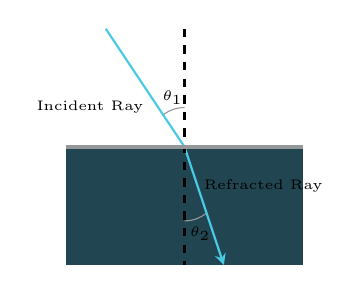
\begin{tikzpicture}
			\fill[p6!20!pag] (-1.5,0) rectangle (1.5, -1.5);

			\draw[pag!50] (0,0.5) arc (90:130:0.44);
			\draw[pag!50] (0,-0.94) arc (270:310:0.44);

			\draw[p4,thick] (-1,1.5) -- (0,0);

			\draw[p4,thick, {stealth}-] (0.5,-1.5) -- (0,0);

			\draw[thick, dashed] (0,1.5) -- (0,-1.5);
			\node at (-0.15,0.63) {\tiny$\theta_1$};
			\node at (0.2,-1.1) {\tiny$\theta_2$};
			\node at (-1.2,0.5) {\tiny Incident Ray};
			\node at (1,-0.5) {\tiny Refracted Ray};

			\draw[ultra thick, pag!50] (-1.5,0) -- (1.5,0);
		\end{tikzpicture}

	\end{minipage}

\end{figure}
\vspace{10pt}
\hspace{-15pt}\begin{minipage}{0.56\textwidth}
	\textbf{Refractive Index} - The refractive index of a medium is the speed of light in a vacuum, divided by the speed of light in that medium. Since the speeds in air and a vacuum are close, $n_{air}\approx 1$. On the right are some speeds of light.
	\begin{center}
		\fbox{$n=\frac{c}{v}=\frac{2.998\cdot10^8}{v}$}
	\end{center}
\end{minipage}
\hspace{15pt}\begin{minipage}{0.4\textwidth}
	\centering
	\begin{center}
		\vspace{-20pt}
		Speed of Light in Different Media
		\renewcommand{\arraystretch}{1.2}
		\arrayrulecolor{pag!93}
		\begin{tabular}{|c|c|}
			\hline
			\rowcolor{pag!90}
			\textbf{Medium} & \textbf{Speed (m/s)}                  \\
			\hline
			Vacuum          & $c = 2.998 \times 10^8$               \\
			\hline
			Air             & $v = 2.997 \times 10^8$ (approx. $c$) \\
			\hline
			Glass           & $v \approx 2 \times 10^8$ (variable)  \\
			\hline
		\end{tabular}
	\end{center}
\end{minipage}

\vspace{20pt}
\begin{figure}[h]
	\begin{minipage}{0.78\textwidth}
		\textbf{Critical Angle} - When the angle of refraction, or $\theta_2$ is greater then $90^{\circ}$, the light ray is actually reflected, following normal rules of reflection. To find the critical angle, you can use the formula below. This is called \textbf{total internal reflection}. This can only happen when a light ray is leaving a more dense material, as that is when it bends away from the normal.\\
		\vspace{-10pt}
		\begin{center}
			\fbox{$\theta_c=\sin^{-1}\left(\frac{n_2}{n_1}\right)$}
		\end{center}

	\end{minipage}
	\begin{minipage}{0.1\textwidth}
		\vspace{-20pt}
		\hspace{5pt}	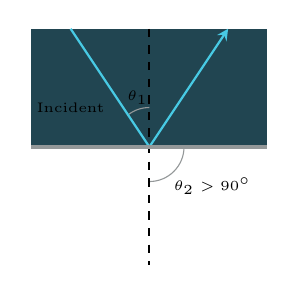
\begin{tikzpicture}
			\fill[p6!20!pag] (-1.5,0) rectangle (1.5, 1.5);

			\draw[pag!50] (0,0.5) arc (90:130:0.44);
			\draw[pag!50] (0,-0.44) arc (270:360:0.44);

			\draw[p4,thick] (-1,1.5) -- (0,0);

			\draw[p4,thick, {stealth}-] (1,1.5) -- (0,0);

			\draw[thick, dashed] (0,1.5) -- (0,-1.5);
			\node at (-0.15,0.63) {\tiny$\theta_1$};
			\node at (0.8,-0.5) {\tiny$\theta_2>90^{\circ}$};
			\node at (-1,0.5) {\tiny Incident};

			\draw[ultra thick, pag!50] (-1.5,0) -- (1.5,0);
		\end{tikzpicture}

	\end{minipage}

\end{figure}

\vspace{10pt}
\hspace{-15pt}\begin{minipage}{0.98\textwidth}
	\textbf{Total Internal Reflection} - Total internal reflection is used for a variety of things. One of these is fiber optics, where information is transmitted via light traveling through a tube with no imperfections (imperfections cause the light to bleed out). The reason why diamonds tend to sparkle is because the refractive index is very high, leading to a very low critical angle. In turn, it can capture light from many different angles and bounce it around.
	\vspace{15pt}
\end{minipage}

\begin{figure}[h]
	\begin{minipage}{0.725\textwidth}
		\textbf{Approximation} - For now, we assume that all the light that goes through the interface is refracted or reflected completely, however, in reality, the part of the light is always reflected, until it hits the critical angle. This will become more important later on. When a ray is incident past its critical angle, all the light will be reflected.\\

	\end{minipage}
	\begin{minipage}{0.1\textwidth}
		\vspace{-20pt}
		\hspace{5pt}	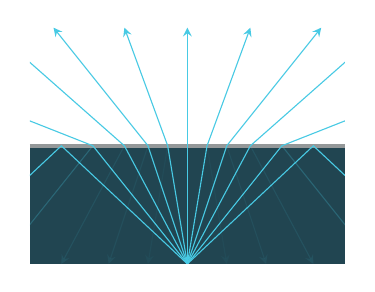
\begin{tikzpicture}
			\fill[p6!20!pag] (-2,0) rectangle (2, -1.5);

			\draw[ultra thick, pag!50] (-2,0) -- (2,0);

			\coordinate (wow) at (0,-1.5);

			\clip (-2,-1.5) rectangle (2,1.5);

			\draw[p4, -{stealth}] (wow) -- (-0.25,0) -- (-0.8,1.5);
			\draw[p4, opacity=0.05, -{stealth}] (-0.25,0) -- (-0.5,-1.5);

			\draw[p4, -{stealth}] (wow) -- (-0.5,0) -- (-1.7,1.5);
			\draw[p4, opacity=0.08, -{stealth}] (-0.5,0) -- (-1,-1.5);

			\draw[p4, -{stealth}] (wow) -- (-0.8,0) -- (-2.5,1.5);
			\draw[p4, opacity=0.1, -{stealth}] (-0.8,0) -- (-1.6,-1.5);

			\draw[p4, -{stealth}] (wow) -- (-1.2,0) -- (-5,1.5);
			\draw[p4, opacity=0.25, -{stealth}] (-1.2,0) -- (-2.4,-1.5);

			\draw [p4, -{stealth}] (wow) -- (-1.6,0) -- (-3.2,-1.5);

			\draw [p4, -{stealth}] (0,-1.5) -- (0,1.5);
			\draw[p4, -{stealth}] (wow) -- (0.25,0) -- (0.8,1.5);
			\draw[p4, opacity=0.05, -{stealth}] (0.25,0) -- (0.5,-1.5);

			\draw[p4, -{stealth}] (wow) -- (0.5,0) -- (1.7,1.5);
			\draw[p4, opacity=0.08, -{stealth}] (0.5,0) -- (1,-1.5);

			\draw[p4, -{stealth}] (wow) -- (0.8,0) -- (2.5,1.5);
			\draw[p4, opacity=0.1, -{stealth}] (0.8,0) -- (1.6,-1.5);

			\draw[p4] (wow) -- (1.2,0) -- (5,1.5);
			\draw[p4, opacity=0.25, -{stealth}] (1.2,0) -- (2.4,-1.5);

			\draw [p4, -{stealth}] (wow) -- (1.6,0) -- (3.2,-1.5);

		\end{tikzpicture}

	\end{minipage}

\end{figure}
\vspace{10pt}

\begin{figure}[h]
	\begin{minipage}{0.62\textwidth}
		\textbf{Converging Lenses} - In converging lenses, the lenses is two convex mirrors put side by side. When a ray of light passes through a concave lens parallel to the central axis, the ray is reflected through the focus, which is positive, but on the opposite side of the incident ray. \\

	\end{minipage}
	\begin{minipage}{0.1\textwidth}
		\vspace{-20pt}

		\newcommand{\convgyscale}{1}
		\newcommand{\convgscale}{0.474}
		\hspace*{10pt}\begin{tikzpicture}[scale=\convgscale, yscale=\convgyscale]
			\begin{scope}[xscale=1]
				\newcommand{\odistance}{2.9}
				\newcommand{\convheight}{2.5}
				\newcommand{\convwidth}{8}
				\newcommand{\lfocus}{2}
				\newcommand{\rfocus}{-2}

				\fill (\lfocus,0) circle (2pt);
				\fill (\rfocus,0) circle (1.5pt);
				\node at (\lfocus,-0.7) {$f$};

				% Axis Lines

				% Define lens parameters
				\def\lensRadius{20} % radius of the lens
				\def\lensHeight{2.5} % half height of the lens

				% Calculate arc start and end points
				\def\startAngle{asin(\lensHeight/\lensRadius)}
				\def\endAngle{180-\startAngle}

				\fill[p4!15!pag] (0,\lensHeight) arc[start angle=\startAngle, end angle=-\startAngle, radius=\lensRadius] --
				(0,\lensHeight) arc[start angle=180-\startAngle, end angle=180+\startAngle, radius=\lensRadius] -- cycle;

				% Draw the two arcs for the lens
				\draw[pag!50] (0,\lensHeight) arc[start angle=\startAngle, end angle=-\startAngle, radius=\lensRadius];
				\draw [pag!50] (0,\lensHeight) arc[start angle=180-\startAngle, end angle=180+\startAngle, radius=\lensRadius];

				\draw [dashed] (-6,0) -- (5,0);

				% Global macro to store the slope
				\newcommand{\currentslope}{}
				% Define the findslope command
				\newcommand{\findslope}[2]{
					\pgfmathsetmacro{\currentslope}{(#2)/(#1 -\lfocus)} % Calculate slope
					% Handling division by zero or near-zero differences
					\pgfmathparse{abs(#1 - \lfocus)<0.001 ? "\infty" : \currentslope} % Check for division by zero
					\global\let\currentslope\pgfmathresult % Store the result globally
				}

				\newcommand{\drawray}[2]{

					\newcommand{\oheight}{#1}

					\pgfmathsetmacro{\xValue}{((1/\lfocus)-(1/\odistance))^(-1)}
					\pgfmathsetmacro{\yValue}{(-\xValue*\oheight)/\odistance}
					\coordinate (image) at (-\xValue, \yValue);
					\coordinate (object) at (\odistance, \oheight);

					\findslope{\odistance}{\oheight}
					\let\focusslope\currentslope % Copy the value to \slopeA

					\draw[p#2,{stealth}-] (\odistance,\oheight) -- (0,{\oheight -((\odistance)*(\focusslope))});
					\draw[p#2,{stealth}-] (\odistance,\oheight) -- (0,{\oheight -((\odistance)*(\focusslope))});
					\draw[p#2,] (0,{\oheight -((\odistance)*(\focusslope))}) -- (image);
					\draw[p#2, {stealth}-] (-3,{\oheight -((\odistance)*(\focusslope))}) -- (image);
					\draw[p#2, {stealth}-] (-0.3,{\oheight -((\odistance)*(\focusslope))}) -- (image);

				}

				\newcounter{shadeCounterb}
				\setcounter{shadeCounterb}{2} % Initialize the counter to 1 (for the first shade)

				\foreach \abc in {-1,-0.5,0,0.5,1}{
						\drawray{\abc}{\theshadeCounterb} % Use the current value of the counter for the shade
						\addtocounter{shadeCounterb}{1} % Increment the counter by 2 for the next shade
					}

				\fill (\lfocus,0) circle (2pt);
			\end{scope}

		\end{tikzpicture}

	\end{minipage}

\end{figure}
\vspace{10pt}

\hspace{-15pt}\begin{minipage}{0.62\textwidth}
	\textbf{Diverging Lenses} - Diverging lenses are very similar, except a incident ray parallel to the central axis will refract along the line made between the focus, the point the ray enters the mirror. The focus in this case is negative, as it is virtual. \\

\end{minipage}
\begin{minipage}{0.1\textwidth}
	\vspace{-20pt}

	\newcommand{\convgyscale}{1}
	\newcommand{\convgscale}{0.474}
	\hspace*{10pt}\begin{tikzpicture}[scale=\convgscale, yscale=\convgyscale]
		\begin{scope}[xscale=-1]
			\newcommand{\odistance}{7}
			\newcommand{\convheight}{2.5}
			\newcommand{\convwidth}{8}
			\newcommand{\lfocus}{4}
			\newcommand{\rfocus}{-4}
			\newcommand{\wellhere}{-2.6}

			\fill (\lfocus,0) circle (2pt);
			\fill (\rfocus,0) circle (1.5pt);
			\node at (\lfocus,-0.7) {$f$};

			% Axis Lines

			% Define lens parameters
			\def\lensRadius{2.502} % radius of the arcs forming the lens
			\def\lensHeight{2.5} % half height of the lens
			\def\lensWidth{0.1} % thickness of the lens at the center

			% Calculate the horizontal distance from the origin to the arc centers
			% This distance is based on the lens height and radius, using the Pythagorean theorem
			\pgfmathsetmacro{\arcCenterDistance}{sqrt(\lensRadius*\lensRadius - \lensHeight*\lensHeight)}

			% Draw the left arc of the diverging lens
			\draw[pag!50, fill=p4!15!pag]
			(-\arcCenterDistance-\lensWidth, -\lensHeight)
			arc[start angle=-90, end angle=90, x radius=\lensWidth, y radius=\lensHeight]
			-- (\arcCenterDistance+\lensWidth, \lensHeight)
			arc[start angle=90, delta angle=180, x radius=\lensWidth, y radius=\lensHeight]
			-- cycle;
			\draw[dashed] (-4.5,0) -- (4,0);

			\newcommand{\drawray}[2]{

			\draw [pag!60, dashed, thin] (\lfocus, 0) -- (0,#1);
			\draw[p#2,-{stealth}] (\odistance,#1) -- (0,#1) -- (\wellhere, {#1+(\wellhere*(-#1/\lfocus))});

			}

			\newcounter{shadeCounterc}
			\setcounter{shadeCounterc}{1} % Initialize the counter to 1 (for the first shade)

			\foreach \abc in {-1.5,-1,-0.5,0,0.5,1,1.5}{
					\drawray{\abc}{\theshadeCounterc} % Use the current value of the counter for the shade
					\addtocounter{shadeCounterc}{1} % Increment the counter by 2 for the next shade
				}

		\end{scope}

	\end{tikzpicture}
\end{minipage}

\vspace{12pt}
\hspace{-15pt}\begin{minipage}{0.98\textwidth}
	\textbf{Thin Lens Approximation} - Again, we make an approximation when dealing with lenses. If you think about it, a ray of light entering the lens will a slightly refracted slope as it travels through the lens. In turn, we a assume the lens is very thin, allowing us to use our formulas.
	\vspace{15pt}
\end{minipage}
\vspace{10pt}

 \textbf{Converging Lens Ray Diagrams} - When drawing ray diagrams, you only have 3 main rays to consider, as seen below. When the object is beyond the focal point, the image will be inverted, and real. We assume a image to be real when it is on the opposite side of the lens that the object is on. When the object passes the focal point, the image is upright and virtual. The focus is \textbf{positive}.
\vspace{10pt}

\newcommand{\convgyscale}{1}
\newcommand{\convgscale}{0.474}
\hspace{-15pt}\fcolorbox{\rbcolor}{\rbocolor}{\begin{tikzpicture}[scale=\convgscale, yscale=\convgyscale]
		\begin{scope}[xscale=-1]
			\newcommand{\odistance}{7.5}
			\newcommand{\oheight}{1}
			\newcommand{\convheight}{2.5}
			\newcommand{\convwidth}{8}
			\newcommand{\lfocus}{2}
			\newcommand{\rfocus}{-2}

			\fill (\lfocus,0) circle (1.5pt) node[below] {\small$f$};
			\fill (\rfocus,0) circle (1.5pt) node[below] {\small$f$};
			\fill (2*\lfocus,0) circle (1.5pt) node[below] {\textcolor{pag!40}{\tiny$2f$}};
			\fill (2*\rfocus,0) circle (1.5pt) node[below] {\textcolor{pag!40}{\tiny$2f$}};
			% Axis Lines

			% Axis Lines
			\draw[opacity=0] (-\convwidth,-\convheight) rectangle (\convwidth,\convheight);

			% Define lens parameters
			\def\lensRadius{20} % radius of the lens
			\def\lensHeight{2.5} % half height of the lens

			% Calculate arc start and end points
			\def\startAngle{asin(\lensHeight/\lensRadius)}
			\def\endAngle{180-\startAngle}

			\fill[p4!15!pag] (0,\lensHeight) arc[start angle=\startAngle, end angle=-\startAngle, radius=\lensRadius] --
			(0,\lensHeight) arc[start angle=180-\startAngle, end angle=180+\startAngle, radius=\lensRadius] -- cycle;

			% Draw the two arcs for the lens
			\draw[pag!50] (0,\lensHeight) arc[start angle=\startAngle, end angle=-\startAngle, radius=\lensRadius];
			\draw [pag!50] (0,\lensHeight) arc[start angle=180-\startAngle, end angle=180+\startAngle, radius=\lensRadius];

			\draw [dashed] (-8,0) -- (8,0);

			\pgfmathsetmacro{\xValue}{((1/\lfocus)-(1/\odistance))^(-1)}
			\pgfmathsetmacro{\yValue}{(-\xValue*\oheight)/\odistance}
			\coordinate (image) at (-\xValue, \yValue);
			\coordinate (object) at (\odistance, \oheight);
			% Global macro to store the slope

			% Define the findslope command
			\newcommand{\findslope}[2]{
				\pgfmathsetmacro{\currentslope}{(#2)/(#1 -\lfocus)} % Calculate slope
				% Handling division by zero or near-zero differences
				\pgfmathparse{abs(#1 - \lfocus)<0.001 ? "\infty" : \currentslope} % Check for division by zero
				\global\let\currentslope\pgfmathresult % Store the result globally
			}

			\findslope{\odistance}{\oheight}
			\let\focusslope\currentslope % Copy the value to \slopeA

			\draw [ultra thick, pag!40] (\odistance, 0) -- (object);
			\draw [ultra thick, pag!80] (-\xValue,0) -- (image);

			\draw[p3] (object) -- (0,{\oheight -((\odistance)*(\focusslope))});
			\draw[p3] (0,{\oheight -((\odistance)*(\focusslope))}) -- (image);

			\draw[p4] (object) -- (0,\oheight);
			\draw[p4] (0,\oheight) -- (image);

			\fill (image) circle (2pt);

			\draw[p7] (object) -- (image);

		\end{scope}

	\end{tikzpicture}}
\hspace{20pt}\fcolorbox{\rbcolor}{\rbocolor}{\begin{tikzpicture}[scale=\convgscale, yscale=\convgyscale]
		\begin{scope}[xscale=-1]
			\newcommand{\odistance}{5.5}
			\newcommand{\oheight}{1}
			\newcommand{\convheight}{2.5}
			\newcommand{\convwidth}{8}
			\newcommand{\lfocus}{2}
			\newcommand{\rfocus}{-2}

			\fill (\lfocus,0) circle (1.5pt) node[below] {\small$f$};
			\fill (\rfocus,0) circle (1.5pt) node[below] {\small$f$};
			\fill (2*\lfocus,0) circle (1.5pt) node[below] {\textcolor{pag!40}{\tiny$2f$}};
			\fill (2*\rfocus,0) circle (1.5pt) node[below] {\textcolor{pag!40}{\tiny$2f$}};
			% Axis Lines

			% Axis Lines
			\draw[opacity=0] (-\convwidth,-\convheight) rectangle (\convwidth,\convheight);
			\draw [dashed] (-8,0) -- (8,0);

			% Define lens parameters
			\def\lensRadius{20} % radius of the lens
			\def\lensHeight{2.5} % half height of the lens

			% Calculate arc start and end points
			\def\startAngle{asin(\lensHeight/\lensRadius)}
			\def\endAngle{180-\startAngle}

			\fill[p4!15!pag] (0,\lensHeight) arc[start angle=\startAngle, end angle=-\startAngle, radius=\lensRadius] --
			(0,\lensHeight) arc[start angle=180-\startAngle, end angle=180+\startAngle, radius=\lensRadius] -- cycle;

			% Draw the two arcs for the lens
			\draw[pag!50] (0,\lensHeight) arc[start angle=\startAngle, end angle=-\startAngle, radius=\lensRadius];
			\draw [pag!50] (0,\lensHeight) arc[start angle=180-\startAngle, end angle=180+\startAngle, radius=\lensRadius];

			\draw [dashed] (-8,0) -- (8,0);

			\pgfmathsetmacro{\xValue}{((1/\lfocus)-(1/\odistance))^(-1)}
			\pgfmathsetmacro{\yValue}{(-\xValue*\oheight)/\odistance}
			\coordinate (image) at (-\xValue, \yValue);
			\coordinate (object) at (\odistance, \oheight);
			% Global macro to store the slope

			% Define the findslope command
			\newcommand{\findslope}[2]{
				\pgfmathsetmacro{\currentslope}{(#2)/(#1 -\lfocus)} % Calculate slope
				% Handling division by zero or near-zero differences
				\pgfmathparse{abs(#1 - \lfocus)<0.001 ? "\infty" : \currentslope} % Check for division by zero
				\global\let\currentslope\pgfmathresult % Store the result globally
			}

			\findslope{\odistance}{\oheight}
			\let\focusslope\currentslope % Copy the value to \slopeA

			\draw [ultra thick, pag!40] (\odistance, 0) -- (object);
			\draw [ultra thick, pag!80] (-\xValue,0) -- (image);

			\draw[p3] (object) -- (0,{\oheight -((\odistance)*(\focusslope))});
			\draw[p3] (0,{\oheight -((\odistance)*(\focusslope))}) -- (image);

			\draw[p4] (object) -- (0,\oheight);
			\draw[p4] (0,\oheight) -- (image);

			\fill (image) circle (2pt);

			\draw[p7] (object) -- (image);

		\end{scope}

	\end{tikzpicture}}
\vspace{15pt}

\hspace{-15pt}\fcolorbox{\rbcolor}{\rbocolor}{\begin{tikzpicture}[scale=\convgscale, yscale=\convgyscale]
		\begin{scope}[xscale=-1]
			\newcommand{\odistance}{4}
			\newcommand{\oheight}{1}
			\newcommand{\convheight}{2.5}
			\newcommand{\convwidth}{8}
			\newcommand{\lfocus}{2}
			\newcommand{\rfocus}{-2}

			\fill (\lfocus,0) circle (1.5pt) node[below] {\small$f$};
			\fill (\rfocus,0) circle (1.5pt) node[below] {\small$f$};
			\fill (2*\lfocus,0) circle (1.5pt) node[below] {\textcolor{pag!40}{\tiny$2f$}};
			\fill (2*\rfocus,0) circle (1.5pt) node[below] {\textcolor{pag!40}{\tiny$2f$}};
			% Axis Lines
			% Axis Lines
			\draw[opacity=0] (-\convwidth,-\convheight) rectangle (\convwidth,\convheight);

			% Define lens parameters
			\def\lensRadius{20} % radius of the lens
			\def\lensHeight{2.5} % half height of the lens

			% Calculate arc start and end points
			\def\startAngle{asin(\lensHeight/\lensRadius)}
			\def\endAngle{180-\startAngle}

			\fill[p4!15!pag] (0,\lensHeight) arc[start angle=\startAngle, end angle=-\startAngle, radius=\lensRadius] --
			(0,\lensHeight) arc[start angle=180-\startAngle, end angle=180+\startAngle, radius=\lensRadius] -- cycle;

			% Draw the two arcs for the lens
			\draw[pag!50] (0,\lensHeight) arc[start angle=\startAngle, end angle=-\startAngle, radius=\lensRadius];
			\draw [pag!50] (0,\lensHeight) arc[start angle=180-\startAngle, end angle=180+\startAngle, radius=\lensRadius];

			\draw [dashed] (-8,0) -- (8,0);

			\pgfmathsetmacro{\xValue}{((1/\lfocus)-(1/\odistance))^(-1)}
			\pgfmathsetmacro{\yValue}{(-\xValue*\oheight)/\odistance}
			\coordinate (image) at (-\xValue, \yValue);
			\coordinate (object) at (\odistance, \oheight);
			% Global macro to store the slope

			% Define the findslope command
			\newcommand{\findslope}[2]{
				\pgfmathsetmacro{\currentslope}{(#2)/(#1 -\lfocus)} % Calculate slope
				% Handling division by zero or near-zero differences
				\pgfmathparse{abs(#1 - \lfocus)<0.001 ? "\infty" : \currentslope} % Check for division by zero
				\global\let\currentslope\pgfmathresult % Store the result globally
			}

			\findslope{\odistance}{\oheight}
			\let\focusslope\currentslope % Copy the value to \slopeA

			\draw [ultra thick, pag!40] (\odistance, 0) -- (object);
			\draw [ultra thick, pag!80] (-\xValue,0) -- (image);

			\draw[p3] (object) -- (0,{\oheight -((\odistance)*(\focusslope))});
			\draw[p3] (0,{\oheight -((\odistance)*(\focusslope))}) -- (image);

			\draw[p4] (object) -- (0,\oheight);
			\draw[p4] (0,\oheight) -- (image);

			\fill (image) circle (2pt);

			\draw[p7] (object) -- (image);

		\end{scope}

	\end{tikzpicture}}
\hspace{20pt}\fcolorbox{\rbcolor}{\rbocolor}{\begin{tikzpicture}[scale=\convgscale, yscale=\convgyscale]
		\begin{scope}[xscale=-1]
			\newcommand{\odistance}{2.9}
			\newcommand{\oheight}{1}
			\newcommand{\convheight}{2.5}
			\newcommand{\convwidth}{8}
			\newcommand{\lfocus}{2}
			\newcommand{\rfocus}{-2}

			\fill (\lfocus,0) circle (1.5pt) node[below] {\small$f$};
			\fill (\rfocus,0) circle (1.5pt) node[below] {\small$f$};
			\fill (2*\lfocus,0) circle (1.5pt) node[below] {\textcolor{pag!40}{\tiny$2f$}};
			\fill (2*\rfocus,0) circle (1.5pt) node[below] {\textcolor{pag!40}{\tiny$2f$}};
			% Axis Lines

			% Axis Lines
			\draw[opacity=0] (-\convwidth,-\convheight) rectangle (\convwidth,\convheight);
			\draw [dashed] (-8,0) -- (8,0);

			% Define lens parameters
			\def\lensRadius{20} % radius of the lens
			\def\lensHeight{2.5} % half height of the lens

			% Calculate arc start and end points
			\def\startAngle{asin(\lensHeight/\lensRadius)}
			\def\endAngle{180-\startAngle}

			\clip (-\convwidth,-\convheight) rectangle (\convwidth,\convheight);

			\fill[p4!15!pag] (0,\lensHeight) arc[start angle=\startAngle, end angle=-\startAngle, radius=\lensRadius] --
			(0,\lensHeight) arc[start angle=180-\startAngle, end angle=180+\startAngle, radius=\lensRadius] -- cycle;

			% Draw the two arcs for the lens
			\draw[pag!50] (0,\lensHeight) arc[start angle=\startAngle, end angle=-\startAngle, radius=\lensRadius];
			\draw [pag!50] (0,\lensHeight) arc[start angle=180-\startAngle, end angle=180+\startAngle, radius=\lensRadius];

			\draw [dashed] (-8,0) -- (8,0);

			\pgfmathsetmacro{\xValue}{((1/\lfocus)-(1/\odistance))^(-1)}
			\pgfmathsetmacro{\yValue}{(-\xValue*\oheight)/\odistance}
			\coordinate (image) at (-\xValue, \yValue);
			\coordinate (object) at (\odistance, \oheight);
			% Global macro to store the slope

			% Define the findslope command
			\newcommand{\findslope}[2]{
				\pgfmathsetmacro{\currentslope}{(#2)/(#1 -\lfocus)} % Calculate slope
				% Handling division by zero or near-zero differences
				\pgfmathparse{abs(#1 - \lfocus)<0.001 ? "\infty" : \currentslope} % Check for division by zero
				\global\let\currentslope\pgfmathresult % Store the result globally
			}

			\findslope{\odistance}{\oheight}
			\let\focusslope\currentslope % Copy the value to \slopeA

			\draw [ultra thick, pag!40] (\odistance, 0) -- (object);
			\draw [ultra thick, pag!80] (-\xValue,0) -- (image);

			\draw[p3] (object) -- (0,{\oheight -((\odistance)*(\focusslope))});
			\draw[p3] (0,{\oheight -((\odistance)*(\focusslope))}) -- (image);

			\draw[p4] (object) -- (0,\oheight);
			\draw[p4] (0,\oheight) -- (image);

			\fill (image) circle (2pt);

			\draw[p7] (object) -- (image);

		\end{scope}

	\end{tikzpicture}}
\vspace{15pt}

\hspace{-15pt}\fcolorbox{\rbcolor}{\rbocolor}{\begin{tikzpicture}[scale=\convgscale, yscale=\convgyscale]
		\begin{scope}[xscale=-1]
			\newcommand{\odistance}{1.55}
			\newcommand{\oheight}{0.5}
			\newcommand{\convheight}{2.5}
			\newcommand{\convwidth}{8}
			\newcommand{\lfocus}{2}
			\newcommand{\rfocus}{-2}

			\fill (\lfocus,0) circle (1.5pt) node[below] {\small$f$};
			\fill (\rfocus,0) circle (1.5pt) node[below] {\small$f$};
			\fill (2*\lfocus,0) circle (1.5pt) node[below] {\textcolor{pag!40}{\tiny$2f$}};
			\fill (2*\rfocus,0) circle (1.5pt) node[below] {\textcolor{pag!40}{\tiny$2f$}};
			% Axis Lines

			% Axis Lines
			\draw[opacity=0] (-\convwidth,-\convheight) rectangle (\convwidth,\convheight);
			\draw [dashed] (-8,0) -- (8,0);

			% Define lens parameters
			\def\lensRadius{20} % radius of the lens
			\def\lensHeight{2.5} % half height of the lens

			% Calculate arc start and end points
			\def\startAngle{asin(\lensHeight/\lensRadius)}
			\def\endAngle{180-\startAngle}

			\clip (-\convwidth,-\convheight) rectangle (\convwidth,\convheight);

			\fill[p4!15!pag] (0,\lensHeight) arc[start angle=\startAngle, end angle=-\startAngle, radius=\lensRadius] --
			(0,\lensHeight) arc[start angle=180-\startAngle, end angle=180+\startAngle, radius=\lensRadius] -- cycle;

			% Draw the two arcs for the lens
			\draw[pag!50] (0,\lensHeight) arc[start angle=\startAngle, end angle=-\startAngle, radius=\lensRadius];
			\draw [pag!50] (0,\lensHeight) arc[start angle=180-\startAngle, end angle=180+\startAngle, radius=\lensRadius];

			\draw [dashed] (-8,0) -- (8,0);

			\pgfmathsetmacro{\xValue}{((1/\lfocus)-(1/\odistance))^(-1)}
			\pgfmathsetmacro{\yValue}{(-\xValue*\oheight)/\odistance}
			\coordinate (image) at (-\xValue, \yValue);
			\coordinate (object) at (\odistance, \oheight);
			% Global macro to store the slope

			% Define the findslope command
			\newcommand{\findslope}[2]{
				\pgfmathsetmacro{\currentslope}{(#2)/(#1 -\lfocus)} % Calculate slope
				% Handling division by zero or near-zero differences
				\pgfmathparse{abs(#1 - \lfocus)<0.001 ? "\infty" : \currentslope} % Check for division by zero
				\global\let\currentslope\pgfmathresult % Store the result globally
			}

			\findslope{\odistance}{\oheight}
			\let\focusslope\currentslope % Copy the value to \slopeA

			\draw [ultra thick, pag!40] (\odistance, 0) -- (object);
			\draw [ultra thick, pag!80] (-\xValue,0) -- (image);

			\draw[p3] (object) -- (0,{\oheight -((\odistance)*(\focusslope))});
			\draw[pag!60, thin, dashed] (0,{\oheight -((\odistance)*(\focusslope))}) -- (image);
			\draw[p3, -{stealth}] (0,{\oheight -((\odistance)*(\focusslope))}) -- (\rfocus,{\oheight -((\odistance)*(\focusslope))});

			\draw[p4] (object) -- (0,\oheight);
			\draw[pag!60, thin, dashed] (0,\oheight) -- (image);
			\draw[p4, -{stealth}] (0,\oheight) -- (\rfocus,0);

			\fill (image) circle (2pt);

			\draw[pag!60, thin, dashed] (object) -- (image);

			\draw[p7, -{stealth}] (object) -- (\rfocus,{ (\odistance-(\odistance-\lfocus))*(-1*(\oheight/\odistance))});

		\end{scope}

	\end{tikzpicture}}
\hspace{20pt}\fcolorbox{\rbcolor}{\rbocolor}{\begin{tikzpicture}[scale=\convgscale, yscale=\convgyscale]
		\begin{scope}[xscale=-1]
			\newcommand{\odistance}{1.2}
			\newcommand{\oheight}{0.5}
			\newcommand{\convheight}{2.5}
			\newcommand{\convwidth}{8}
			\newcommand{\lfocus}{2}
			\newcommand{\rfocus}{-2}

			\fill (\lfocus,0) circle (1.5pt) node[below] {\small$f$};
			\fill (\rfocus,0) circle (1.5pt) node[below] {\small$f$};
			\fill (2*\lfocus,0) circle (1.5pt) node[below] {\textcolor{pag!40}{\tiny$2f$}};
			\fill (2*\rfocus,0) circle (1.5pt) node[below] {\textcolor{pag!40}{\tiny$2f$}};
			% Axis Lines

			% Axis Lines
			\draw[opacity=0] (-\convwidth,-\convheight) rectangle (\convwidth,\convheight);
			\draw [dashed] (-8,0) -- (8,0);

			% Define lens parameters
			\def\lensRadius{20} % radius of the lens
			\def\lensHeight{2.5} % half height of the lens

			% Calculate arc start and end points
			\def\startAngle{asin(\lensHeight/\lensRadius)}
			\def\endAngle{180-\startAngle}

			\clip (-\convwidth,-\convheight) rectangle (\convwidth,\convheight);

			\fill[p4!15!pag] (0,\lensHeight) arc[start angle=\startAngle, end angle=-\startAngle, radius=\lensRadius] --
			(0,\lensHeight) arc[start angle=180-\startAngle, end angle=180+\startAngle, radius=\lensRadius] -- cycle;

			% Draw the two arcs for the lens
			\draw[pag!50] (0,\lensHeight) arc[start angle=\startAngle, end angle=-\startAngle, radius=\lensRadius];
			\draw [pag!50] (0,\lensHeight) arc[start angle=180-\startAngle, end angle=180+\startAngle, radius=\lensRadius];

			\draw [dashed] (-8,0) -- (8,0);

			\pgfmathsetmacro{\xValue}{((1/\lfocus)-(1/\odistance))^(-1)}
			\pgfmathsetmacro{\yValue}{(-\xValue*\oheight)/\odistance}
			\coordinate (image) at (-\xValue, \yValue);
			\coordinate (object) at (\odistance, \oheight);
			% Global macro to store the slope

			% Define the findslope command
			\newcommand{\findslope}[2]{
				\pgfmathsetmacro{\currentslope}{(#2)/(#1 -\lfocus)} % Calculate slope
				% Handling division by zero or near-zero differences
				\pgfmathparse{abs(#1 - \lfocus)<0.001 ? "\infty" : \currentslope} % Check for division by zero
				\global\let\currentslope\pgfmathresult % Store the result globally
			}

			\findslope{\odistance}{\oheight}
			\let\focusslope\currentslope % Copy the value to \slopeA

			\draw [ultra thick, pag!40] (\odistance, 0) -- (object);
			\draw [ultra thick, pag!80] (-\xValue,0) -- (image);

			\draw[p3] (object) -- (0,{\oheight -((\odistance)*(\focusslope))});
			\draw[pag!60, thin, dashed] (0,{\oheight -((\odistance)*(\focusslope))}) -- (image);
			\draw[p3, -{stealth}] (0,{\oheight -((\odistance)*(\focusslope))}) -- (\rfocus,{\oheight -((\odistance)*(\focusslope))});

			\draw[p4] (object) -- (0,\oheight);
			\draw[pag!60, thin, dashed] (0,\oheight) -- (image);
			\draw[p4, -{stealth}] (0,\oheight) -- (\rfocus,0);

			\fill (image) circle (2pt);

			\draw[pag!60, thin, dashed] (object) -- (image);

			\draw[p7, -{stealth}] (object) -- (\rfocus,{ (\odistance-(\odistance-\lfocus))*(-1*(\oheight/\odistance))});

		\end{scope}

	\end{tikzpicture}}

\vspace{20pt}
\textbf{Diverging Lens Ray Diagrams} - When drawing diverging lens diagrams, things are much simpler. The image is always virtual and upright. The image will always be larger then object. The focal length is considered to be negative.
\vspace{10pt}

\hspace{-15pt}\fcolorbox{\rbcolor}{\rbocolor}{\begin{tikzpicture}[scale=\convgscale, yscale=\convgyscale]
		\begin{scope}[xscale=-1]
			\newcommand{\odistance}{7}
			\newcommand{\oheight}{2}
			\newcommand{\convheight}{2.5}
			\newcommand{\convwidth}{8}
			\newcommand{\lfocus}{2}
			\newcommand{\rfocus}{-2}
			\newcommand{\wellhere}{-4}

			\fill (\lfocus,0) circle (1.5pt) node[below] {\small$f$};
			\fill (\rfocus,0) circle (1.5pt) node[below] {\small$f$};
			\fill (2*\lfocus,0) circle (1.5pt) node[below] {\textcolor{pag!40}{\tiny$2f$}};
			% Axis Lines

			% Axis Lines
			\draw[opacity=0] (-2,-\convheight) rectangle (\convwidth,\convheight);
			\draw [dashed] (-2,0) -- (8,0);

			\clip (-2,-\convheight) rectangle (\convwidth,\convheight);

			% Define lens parameters
			\def\lensRadius{2.502} % radius of the arcs forming the lens
			\def\lensHeight{2.5} % half height of the lens
			\def\lensWidth{0.1} % thickness of the lens at the center

			% Calculate the horizontal distance from the origin to the arc centers
			% This distance is based on the lens height and radius, using the Pythagorean theorem
			\pgfmathsetmacro{\arcCenterDistance}{sqrt(\lensRadius*\lensRadius - \lensHeight*\lensHeight)}

			% Draw the left arc of the diverging lens
			\draw[pag!50, fill=p4!15!pag]
			(-\arcCenterDistance-\lensWidth, -\lensHeight)
			arc[start angle=-90, end angle=90, x radius=\lensWidth, y radius=\lensHeight]
			-- (\arcCenterDistance+\lensWidth, \lensHeight)
			arc[start angle=90, delta angle=180, x radius=\lensWidth, y radius=\lensHeight]
			-- cycle;

			\pgfmathsetmacro{\xValue}{((1/\rfocus)-(1/\odistance))^(-1)}
			\pgfmathsetmacro{\yValue}{(\xValue*\oheight)/\odistance}
			\coordinate (image) at (-\xValue, -\yValue);
			\coordinate (object) at (\odistance, \oheight);

			\draw [ultra thick, pag!40] (\odistance, 0) -- (object);
			\draw [ultra thick, pag!80] (-\xValue,0) -- (image);

			\draw [p2] (object) -- (0, \oheight) -- (\wellhere, {\wellhere*(-\oheight/\lfocus)} );
			\draw[dashed, thin, pag!50] (image) -- (0, \oheight);

			\draw[p6] (object) -- (0,-\yValue) -- (\wellhere,-\yValue);
			\draw[dashed, thin, pag!50] (image) -- (0,-\yValue);

			\draw[p4] (object) -- (\wellhere, {\wellhere*(\oheight/\odistance)});

		\end{scope}

	\end{tikzpicture}}
\hspace{11pt}\fcolorbox{\rbcolor}{\rbocolor}{\begin{tikzpicture}[scale=\convgscale, yscale=\convgyscale]
		\begin{scope}[xscale=-1]
			\newcommand{\odistance}{3}
			\newcommand{\oheight}{2}
			\newcommand{\convheight}{2.5}
			\newcommand{\convwidth}{8}
			\newcommand{\lfocus}{2}
			\newcommand{\rfocus}{-2}
			\newcommand{\wellhere}{-4}

			\fill (\lfocus,0) circle (1.5pt) node[below] {\small$f$};
			\fill (\rfocus,0) circle (1.5pt) node[below] {\small$f$};
			\fill (2*\lfocus,0) circle (1.5pt) node[below] {\textcolor{pag!40}{\tiny$2f$}};
			% Axis Lines

			% Axis Lines
			\draw[opacity=0] (-2,-\convheight) rectangle (\convwidth,\convheight);
			\draw [dashed] (-2,0) -- (8,0);

			\clip (-2,-\convheight) rectangle (\convwidth,\convheight);

			% Define lens parameters
			\def\lensRadius{2.502} % radius of the arcs forming the lens
			\def\lensHeight{2.5} % half height of the lens
			\def\lensWidth{0.1} % thickness of the lens at the center

			% Calculate the horizontal distance from the origin to the arc centers
			% This distance is based on the lens height and radius, using the Pythagorean theorem
			\pgfmathsetmacro{\arcCenterDistance}{sqrt(\lensRadius*\lensRadius - \lensHeight*\lensHeight)}

			% Draw the left arc of the diverging lens
			\draw[pag!50, fill=p4!15!pag]
			(-\arcCenterDistance-\lensWidth, -\lensHeight)
			arc[start angle=-90, end angle=90, x radius=\lensWidth, y radius=\lensHeight]
			-- (\arcCenterDistance+\lensWidth, \lensHeight)
			arc[start angle=90, delta angle=180, x radius=\lensWidth, y radius=\lensHeight]
			-- cycle;

			\pgfmathsetmacro{\xValue}{((1/\rfocus)-(1/\odistance))^(-1)}
			\pgfmathsetmacro{\yValue}{(\xValue*\oheight)/\odistance}
			\coordinate (image) at (-\xValue, -\yValue);
			\coordinate (object) at (\odistance, \oheight);

			\draw [ultra thick, pag!40] (\odistance, 0) -- (object);
			\draw [ultra thick, pag!80] (-\xValue,0) -- (image);

			\draw [p2] (object) -- (0, \oheight) -- (\wellhere, {\wellhere*(-\oheight/\lfocus)} );
			\draw[dashed, thin, pag!50] (image) -- (0, \oheight);

			\draw[p6] (object) -- (0,-\yValue) -- (\wellhere,-\yValue);
			\draw[dashed, thin, pag!50] (image) -- (0,-\yValue);

			\draw[p4] (object) -- (\wellhere, {\wellhere*(\oheight/\odistance)});

		\end{scope}

	\end{tikzpicture}}
\hspace{11pt}\fcolorbox{\rbcolor}{\rbocolor}{\begin{tikzpicture}[scale=\convgscale, yscale=\convgyscale]
		\begin{scope}[xscale=-1]
			\newcommand{\odistance}{1}
			\newcommand{\oheight}{2}
			\newcommand{\convheight}{2.5}
			\newcommand{\convwidth}{8}
			\newcommand{\lfocus}{2}
			\newcommand{\rfocus}{-2}
			\newcommand{\wellhere}{-4}

			\fill (\lfocus,0) circle (1.5pt) node[below] {\small$f$};
			\fill (\rfocus,0) circle (1.5pt) node[below] {\small$f$};
			\fill (2*\lfocus,0) circle (1.5pt) node[below] {\textcolor{pag!40}{\tiny$2f$}};
			% Axis Lines

			% Axis Lines
			\draw[opacity=0] (-2,-\convheight) rectangle (\convwidth,\convheight);
			\draw [dashed] (-2,0) -- (8,0);

			\clip (-2,-\convheight) rectangle (\convwidth,\convheight);

			% Define lens parameters
			\def\lensRadius{2.502} % radius of the arcs forming the lens
			\def\lensHeight{2.5} % half height of the lens
			\def\lensWidth{0.1} % thickness of the lens at the center

			% Calculate the horizontal distance from the origin to the arc centers
			% This distance is based on the lens height and radius, using the Pythagorean theorem
			\pgfmathsetmacro{\arcCenterDistance}{sqrt(\lensRadius*\lensRadius - \lensHeight*\lensHeight)}

			% Draw the left arc of the diverging lens
			\draw[pag!50, fill=p4!15!pag]
			(-\arcCenterDistance-\lensWidth, -\lensHeight)
			arc[start angle=-90, end angle=90, x radius=\lensWidth, y radius=\lensHeight]
			-- (\arcCenterDistance+\lensWidth, \lensHeight)
			arc[start angle=90, delta angle=180, x radius=\lensWidth, y radius=\lensHeight]
			-- cycle;

			\pgfmathsetmacro{\xValue}{((1/\rfocus)-(1/\odistance))^(-1)}
			\pgfmathsetmacro{\yValue}{(\xValue*\oheight)/\odistance}
			\coordinate (image) at (-\xValue, -\yValue);
			\coordinate (object) at (\odistance, \oheight);

			\draw [ultra thick, pag!40] (\odistance, 0) -- (object);
			\draw [ultra thick, pag!80] (-\xValue,0) -- (image);

			\draw [p2] (object) -- (0, \oheight) -- (\wellhere, {\wellhere*(-\oheight/\lfocus)} );
			\draw[dashed, thin, pag!50] (image) -- (0, \oheight);

			\draw[p6] (object) -- (0,-\yValue) -- (\wellhere,-\yValue);
			\draw[dashed, thin, pag!50] (image) -- (0,-\yValue);

			\draw[p4] (object) -- (\wellhere, {\wellhere*(\oheight/\odistance)});

		\end{scope}

	\end{tikzpicture}}

\vspace{20pt}
\textbf{Lens Equations} - The equations we use for lenses are exactly the same as the ones for mirrors. The only thing you have to watch out for is the focus, which is negative in diverging mirrors and positive in converging mirrors.\\
\\
\\
\\
\\
\textbf{Lens Maker Equation}

\pagebreak
16.5726 cm

\end{document}